\documentclass[12pt]{article}

\usepackage{amssymb,amsmath,amsfonts,eurosym,geometry,ulem,graphicx,caption,color,setspace,sectsty,comment,footmisc,caption,natbib,pdflscape,subfigure,array,hyperref}
\usepackage{hyperref}
\hypersetup{colorlinks,
citecolor=blue,
linkcolor=magenta
}
\usepackage{multirow}
\usepackage{booktabs}
\usepackage{graphicx}
\usepackage{lscape}
\usepackage{setspace}
\usepackage{tabularx} 
\usepackage{rotating}
\usepackage{tablefootnote}
\usepackage{amssymb}
\usepackage{array}
\usepackage{ragged2e}
\usepackage{nicematrix}
\usepackage{enumitem}
\usepackage{array} 
\usepackage{graphicx}
\usepackage{booktabs}
\usepackage{enumitem}
\usepackage{wasysym}
\usepackage{framed}
\usepackage{pgfgantt}
\usepackage{subfloat}
\usepackage{multirow}
\usepackage{blindtext}
\usepackage{graphicx}
\usepackage{lscape}
\usepackage{colortbl}
\usepackage{caption}

\normalem

\doublespacing
\newtheorem{theorem}{Theorem}
\newtheorem{corollary}[theorem]{Corollary}
\newtheorem{proposition}{Proposition}
\newenvironment{proof}[1][Proof]{\noindent\textbf{#1.} }{\ \rule{0.5em}{0.5em}}

\newtheorem{hyp}{Hypothesis}
\newtheorem{subhyp}{Hypothesis}[hyp]
\renewcommand{\thesubhyp}{\thehyp\alph{subhyp}}
%\renewcommand{\familydefault}{\sfdefault} 
%\usepackage{kpfonts}
%\usepackage[T1]{fontenc}


\geometry{left=1.0in,right=1.0in,top=1.0in,bottom=1.0in}
\bibliographystyle{apalike}%aaai-named

\singlespacing
\title{\textbf{Has financialization changed the impact\\ of macro announcements ?}%\thanks{The authors thank participants at meetings of the Commodity \& Energy Markets Association (2021),  World Finance \& Banking Association (2021), Société canadienne de science  économique (2022), 4th Ethical Finance and Sustainability (EFS) conference (2022), and Multinational Finance Society (2022), at a seminar in Humboldt University Berlin, as well as Alessandro Melone, Jocelyn Grira and Joseph Marks (discussants). For financial support, the authors thank the Social Sciences and Humanities Research Council and the Chaire Industrielle-Alliance Groupe financier. Any remaining errors are ours alone.}}
%J'arrive pas le centrer dans le titre
%\author{Simon-Pierre Boucher\footnote{Corresponding author, PhD student in finance, Université Laval, Quebec City QC Canada G1V 0A6, email:   \texttt{simon-pierre.boucher.1@ulaval.ca}}\and Marie-H{\'e}l{\`e}ne Gagnon\footnote{Professor of Finance and Research Fellow, CRREP, Université Laval, email: \texttt{marie-helene.gagnon@fsa.ulaval.ca}}\and Gabriel J. Power\footnote{IG Wealth Management Chairholder, Professor of Finance and Research Fellow, CRREP and CRIB, Université Laval, email:   \texttt{gabriel.power@fsa.ulaval.ca}}. 
}
%\author{ANONYMOUS VERSION}
\date{ \today \\ First version: June 2021}
\begin{document}
\begin{titlepage}
\maketitle





\begin{abstract}
\noindent 
\singlespacing
%Turmoil in commodity markets can threaten a sustainable energy future.
%The transition to a sustainable energy future requires considerable investments, which can be discouraged by heightened volatility in commodity markets.
 We investigate, using high-frequency data, how financialization has affected the impact of macroeconomic announcements on commodity futures returns and volatility. We find that financialization lessens the impact of macro news on commodity markets, as measured by price drift and volatility changes. This result is consistent with prior literature suggesting that financial participants improve liquidity and price discovery, while reducing volatility. Assuming that traditional market participants prefer stability, our results suggest a beneficial impact of financialization. We further show that the effects of greater participation by swap dealers and money managers differ.%, especially for pro-cyclical commodities such as crude oil and natural gas.

\vspace{0.2in}
\noindent\textbf{Keywords:} commodities, energy, futures,  spillover, financialization, high-frequency, sustainable, commercial, institutional, volatility, macro, announcements, surprise, events\\


\bigskip
\end{abstract}
\setcounter{page}{0}
\thispagestyle{empty}
\end{titlepage}
\pagebreak \newpage




\doublespacing

\section{Introduction} \label{sec:introduction}

%The financialization of commodities appears to have affected in particular the energy sector \citep{Singleton2014}. This is not surprising, given the dependence of our societies on fossil fuels. However, with the growing need for a green energy transition, it is reasonable to believe that financialization will also affect the metals sector as these commodities are used in new technologies (such as electrical car batteries) to achieve this transition. 
 %%INTRO
%Despite all those concerns financialization could be helpful for the development of sustainable energy market.
%If financialization  decreasing volatility, in commo and energy markets, it could foster greater investment in green energy sustianble transition. In fact, real option theory suggests that volatility disoucrages investment. Real option value theory means that volatility discourages investment because of option value of waiting when volatility is higher. Kellogg reference.
%This implies that fostering commodity market stability should improve investment in green energy sustainable transition.
%As more stable commodity markets would plausibly lead to greater investment in greeen transitition energy, it is relevant to investgiate to whether occurred in recent times and its impact on the underlying price distribution as it  as more widrespread market could be a step towards more  Sustainable, affordable and accessible raw energy markets.
%%Carbon markets could help


Since the early 2000s, commodities have gained renewed popularity among non-traditional market participants such as hedge funds and index traders, mainly for diversification or speculative purposes. What is often called the \emph{financialization of commodities} consists of several important market and regulatory changes affecting how commodities (futures, options, swaps and also physicals) are traded by institutional and other non-traditional investors. Such increases in speculation and long-only index positions in commodity markets have been pointed out as being responsible for, respectively, increases in volatility and correlation between different commodities.\footnote{Helpful surveys of this large literature include \citet{boyd2018update} and \citet{cheng2014financialization}.}

The financialization of commodities coincides, however, with a rare commodity bull cycle \cite{humphreys2010great}, that some refer to as a commodity ``supercycle''. Commodity price supercycles are extended periods when commodity prices are substantially above their long-term trend (or below trend, for a bear cycle). According to the Bank of Canada, the last super cycle started in 1996 with a peak around 2011. This supercycle has not officially ended, but the rapid increase in the price of most commodities following the COVID-19 pandemic could potentially bring this cycle to an end. During such periods, traditional market participants have voiced concerns that prices are distorted  away from their fundamental values. For instance, \citet{masters2009testimony} argued  that institutional investors have disrupted commodity markets through the use of investment strategies typically reserved for financial securities. This \emph{Masters hypothesis} has been, however, challenged by empirical research \citep{irwin2011index,irwin2012testing,irwin2012financialization}. According to \citet{cheng2014financialization}, financialization affects commodity futures markets through risk sharing and information discovery. Indeed, investors can either provide liquidity to meet the hedging needs of other traders or consume liquidity when they trade for their own needs \citep{kang2020tale} , thereby influencing liquidity risk. Price discovery in commodity markets is affected by informational frictions in the global supply, demand and inventories of commodities. Indeed, futures markets inform spot or cash markets, which are more decentralized. As a result, financialization could alter how commodity markets incorporate new information.

It is difficult to assess the information that investors possess. A widely-used approach in the literature is to consider macroeconomic announcements as a source of relevant information. The advantage of using this proxy is that we know the exact time when investors will have access to it. Statistical agencies collect, aggregate and release information about various aspects of the macro-economy, providing potentially useful indicators to investors. As a result, there is substantial media coverage when this information is released.

In light of these channels of information discovery, we investigate financialization in commodity markets through the lens of macroeconomic announcement releases and high-frequency data. We assess the extent to which financialization  affects how commodity futures reactions to surprises in macroeconomic announcements. In doing so, we examine the  resolution of uncertainty, market efficiency, and how news are anticipated. Our paper builds on the financial literature on  information transmission in markets. \citet{goldstein2019commodity} show how financial participants in commodity markets affect futures price informativeness, bias, and comovement. Their model predicts that financialization initially improves, but eventually worsens, price efficiency measured through volatility. This paper also relates to \citet{brunetti2016speculators}, who show evidence on the positions held by different types of speculators. They show that hedge funds aid commodity markets by providing additional liquidity, resulting in more efficient prices. In contrast, merchant positions are positively correlated with volatility in crude oil and natural gas markets. 

%%%%%CE PARAGRAPHE EST MOINS PERTINENT POUR  J F Q A???. ON POURRA LE RAJOUTER POUR  E J.
Energy transition shines a new light on financialization as it may prove  helpful to develop sustainable energy markets. For instance, if financialization decreases volatility in commodity and energy markets, it could foster greater investment in energy transition. In fact, real option theory predicts that higher volatility discourages investment because the option value of waiting increases when volatility increases \citep{kellogg2014effect}.  Thus,  stability in commodity markets may foster more investments in the  energy  transition. While most of the focus so far has been  on energy firms, a large demand is also being created for the metals and minerals needed to build renewable energy infrastructures. Moreover, analysts argue that the energy transition will initiate a new commodity supercycle.\footnote{See e.g. J.P. Morgan Asset Management, ``A new supercycle – the clean tech transition and implications for global commodities,'' February 24, 2022. \url{https://am.jpmorgan.com/lu/en/asset-management/per/insights/market-insights/market-updates/on-the-minds-of-investors/clean-energy-investment/}}  These issues relate to the impacts of macroeconomics announcements as this transition may prove to alter the relationship between commodity markets and the real economy. \citet{knuth2018breakthroughs} emphasizes that the gradual shift away from fossil fuels may lessen the impacts of financialization on futures contracts and their relationship with commodity spot prices. Therefore, it is relevant to investigate whether financialization could, through a broadening of the investor base, be a step towards more sustainable, affordable and accessible raw energy markets.
%Carbon markets could help%As more stable commodity markets would plausibly lead to greater investment in  energy transition , i


%CONCLUSION. 
%This paper and the recent body of research suggests that financialization may contribute to sustanability alongside other instruments such as green bonds and portfolio screens for sustainable invvestments.
%
%In the coming years, it will be essential to assess whether the gradual shift away from fossil fuels is lessening the impact of financialization on futures contracts, and the link with commodity spot prices \citep{Knuth2018}.



%%CONTRIBUTION
Our main contribution is to present new insights by bridging the macro announcements and financialization literatures. To better understand the impact of announcements, this literature has moved from daily to high-frequency data, examining  bonds  \citep{andersen2007real, hu2013noise, balduzzi2001economic,lee1995oil, hautsch2011impact, kurov2019price}, stocks \citep{andersen2007real,bernile2016can,kurov2019price} and foreign exchange rates \citep{lee1995oil,andersen2003micro}. But the use of high frequency data is not widespread in commodity futures research. We argue that this literature's use of a lower sampling frequency for futures price returns could explain why no clear answer has emerged concerning volatility \citep{tang2012index,brunetti2016speculators,irwin2012testing,stoll2010commodity,alquist2013role}. Since most of of these studies use daily or monthly data, the resulting sample size is fairly small, which reduces the power of statistical tests \citep{irwin2009devil}.  

Thus, to better measure the impact of financialization, we look at information diffusion in the setting of high-frequency macro announcement releases. With these data, we can measure separately permanent and transitory, news-related shocks on volatility and price returns.
Using high-frequency data further allows us to bypass a traditional criticism of event-study methods, namely that at a daily frequency, the effect of an announcement could easily be attributable to another market event \citep{kothari2007econometrics}. We focus on the US market due to the greater availability of high-frequency data on commodity futures as well as the wealth of distinct macro announcements.

Our second contribution is to consider richer measures of financialization than previously used. Research typically considers sufficient to split the sample into pre- and post-financialization periods, generally using 2004 as the break point \citep{buyukcsahin2010matters, kilian2014role,brunetti2016speculators,irwin2012financialization,stoll2010commodity,alquist2013role}.\footnote{Although the Commodity Futures Trading Commission passed the Commodity Futures Modernization Act in 2000, the literature generally agrees that 2004 marks the beginning of financialization.} While the timing is broadly accepted, using this approach neglects time-varying levels of non-traditional trader activity in the post-financialization period. In addition, we provide deeper economic insights by separately quantifying speculation by fund managers and swap dealers.
%Most previous studies have assumed that financialization started in the early 2000s and that separating the sample into two groups (pre- and post-financialization) is sufficient to capture the impact of this phenomenon \citep{buyukcsahin2010matters, kilian2014role,brunetti2016speculators,irwin2012financialization,stoll2010commodity,alquist2013role}. 
%it is well established that the period of financialization seems to have started in the early-to-mid 2000s


 We summarize our findings as follows: First, we show that financialization contributes to information diffusion and price discovery. The impact of macro announcement surprises is typically dampened when  a given commodity is more affected by financialization. This result suggests that commodity markets are better informed--and macro news generate less of a shock--when commodities are financialized. This outcome should be beneficial to traditional commodity market participants.  This dampening effect  is stronger for pro-cyclical commodities such as crude oil or natural gas. In contrast, the evidence is weaker in the case of gold, a safe haven asset. %This result is particularly relevant for the energy commodity sector. 

Second, we provide a disaggregated analysis by looking at money managers and swap dealers separately. We find that money managers contribute more to price discovery when there is a macro announcement while helping to reduce volatility. This result is consistent with the idea that money managers are more informed investors, given their role in the markets. Swap dealers also contribute to price discovery but are linked to an increase in volatility after macro announcements. Considering all categories of traders, greater levels of financialization overall seem to reduce  volatility in commodity markets. 

Regarding policy implications, our results reject the \citet{masters2009testimony} hypothesis, according to which  financialization increases commodity price instability.  However, when we separate financial traders into two categories, our results allow us to reject  the \citet{masters2009testimony} hypothesis only for money managers. The evidence points a different way for swap dealers, suggesting they may contribute to commodity price instability. Lastly, the robustness tests we perform show that our main findings are robust to the use of alternative volatility measures and to differences in econometric specification.
%and systemic risk%Thus, what we find is consistent with a considerable share of the literature.





%%%%%%%%%%%%%%%%%%%%%%%%%%%%%%%%%%%%%%%%%%%%%%%%%%%%%%%%%%%%%%%%%%%%%%%%%%%%%%%%%%%%%%%%%%%
%%%%%%%%%%%%%%%%%%%%%%%%%%%%%%%%%%%%%%%%%%%%%%%%%%%%%%%%%%%%%%%%%%%%%%%%%%%%%%%%%%%%%%%%%%%

%Include the tex file for Litterature review 

\section{Literature Review}
\subsection{Financialization of Commodities}

The literature has not reached a consensus concerning the impact of financialization on commodity futures prices and volatility. \citet{basak2016model} develop a theoretical model that yields four main findings suggesting a meaningful impact. (i) The prices of all commodity futures increase with financialization and this increase is more significant for futures belonging to the index than for non-indexed futures. (ii) The volatility of both index and non-index futures return increases with financialization. (iii) Correlations between commodity futures returns, as well as equity-commodity correlations, increase with financialization. (iv) Only prices of storable commodities are affected by financialization. Moreover, inventories and prices of storable commodities are higher in the presence of institutional investors than in the benchmark economy, and more so for commodities included in the index.

 In contrast with their sharp theoretical predictions, the empirical evidence is mixed. \citet{tang2012index} show that prices of crude oil prices and other, non-energy commodities have become more correlated as a result of the influence of index funds and the rapid growth of index investments in commodity markets. They argue that when a commodity is included in a benchmark index, its price is no longer determined solely by supply and demand. Rather, it is also determined by other commodities and assets included in the index. Moreover, \citet{singleton2014investor} shows that speculative activity by financial investors creates significant informational frictions such that commodity prices can quickly move away from the value that is justified by fundamentals. He concludes that volatility increases considerably due to financialization, as a result of information friction and prices deviating from economic fundamentals. Using a Granger causality test and forecasting on the error of variance, \citet{yang2005futures} show that when commodity futures trading volume increases, so does the volatility of commodity spot prices. 

However, \citet{stoll2010commodity}  show that inflows and outflows from commodity index investments do not cause significant changes in price and volatility in the Granger sense. Using an arbitrage argument, \citet{hamilton2014risk} show that the positions of commodity traders included in index funds cannot be used to achieve excess returns in  futures markets. In addition, \citet{kilian2014role}  show that several speculative trades can occur in the oil market without observing a significant change in inventory levels, ruling out speculation as being responsible for the boom and bust in the oil market between 2003 and 2008. Several studies similarly conclude that financialization does not increase volatility. \citet{bryant2006causality} reject the hypothesis that speculation and uninformed traders affect the level of volatility. They show that the two theories that would predict this hypothesis, hedging pressure and normal backwardation, are empirically rejected and have no explanatory power. Finally, using a conditional variance measure as well as daily returns on raw material futures, \citet{bohl2013does} show that financialization implies no change in variance.


 Some studies differentiate the impact of different trader types, given their economic motivations. \citet{brunetti2014commodity}  use an equilibrium model and data on trader positions in commodity futures markets to show that index traders provide insurance against price risk.   Closer to this paper, \citet{brunetti2016speculators}  analyze the impact of certain types of speculators in commodity markets from 2005 to 2009. They find that hedge funds allow for faster and more efficient price discovery, resulting in a lower volatility. Furthermore, they find that the positions of swap dealers are not correlated with contemporaneous returns and volatility in the commodity markets.  \textcolor{red}{Table 1} presents a summary of the literature on the influence of financialization and speculation on the volatility of commodity futures returns.
  %However, a consensus has not been reached in the literature.%   As for financialization linked to speculation,   Moreover,  

\subsection{Macroeconomic Announcements}

Other research has examined whether economic conditions can explain some of the more heterogeneous responses across business cycles \citep{boyd2005stock,andersen2003micro}. \citet{boyd2005stock} shows that the impact of announcements related to unemployment has a different impact depending on the economic situation. \citet{andersen2003micro} also find that the stock market reacts to news differently depending on the stage of the business cycle.

Exploiting the fact that high-frequency traders receive the Michigan Consumer Sentiment Index 2 seconds before its official announcement, \citet{hu2017early} show that there is evidence of highly concentrated trading and rapid price discovery occurring within 200 milliseconds. Outside this narrow window, typical investors trade at fully adjusted prices. 

\citet{balduzzi2001economic}  use intraday data from the interdealer government bond market to investigate the effects of scheduled macroeconomic announcements on prices, trading volume, and bid-ask spreads. They find that 17 public news releases, as measured by the surprise in the announced quantity, have a significant impact on the price of at least one of the following instruments: a three-month bill, a two-year note, a 10-year note, and a 30-year bond. In addition, they argue that these effects vary significantly according to maturity. The authors also show that following a macroeconomic announcement, volatility and trade volume increase persistently and significantly.

%(see e.g. cite quelques papiers que j’ai enlevé)
A large literature documents the impact of macroeconomic announcements on stocks \citep{boyd2005stock,andersen2003micro,hu2017early,scholtus2014speed} and bonds \citep{fleming1997moves,fleming1999price,balduzzi2001economic}. In contrast, the commodity literature so far has mostly focused on energy commodities and in particular on OPEC meeting announcements.  \citet{horan2004implied} find that volatility drifts upward as OPEC meetings draw nearer. It decreases  after the first day of the meetings and continues to fall in a 5-day window. \citet{wirl2004impact} assess the influence of OPEC on world oil markets by looking at fifty OPEC meetings from 1984 to 2001. They find that markets does not seem to reflect much about these meetings. \citet{kilian2011energy} run daily frequency regressions of WTI crude oil and U.S. gasoline prices on 30 U.S. macroeconomic announcements from 1983 to 2008. They find no evidence of statistically significant responses for either oil or gasoline.  \citet{gu2018drives} provide an explanation for the pre-announcement price drift in the natural gas market. They show that inventory surprises can be predicted using the difference between the forecast of the historically highly-accurate median analyst and the consensus forecast.

% to U.S. macroeconomic news at daily time horizons.
%vol decr by three percent and by five percent over a five-day window period


In an early study of announcement releases and commodities, \citet{frankel1985commodity}  find, using daily data, that a 1 percentage point positive shock in the money supply leads to a 0.7 percent decline in gold prices. \citet{christie2000macroeconomics} analyzes the sensitivity of gold and silver futures prices over 15-minute intervals to 23 U.S. macroeconomic news announcements from 1992 to 1995. He finds that gold and silver price volatility is higher during days in which there are announcements. \citet{cai2001moves} capture intraday patterns of 5-minute gold price variation using GARCH models around macro announcements. They intraday price effects of announcements to be fewer and less significant for gold than for bonds or currencies.  Likewise, \citet{hess2008commodity} find that CRB and Goldman Sachs commodity indexes are less sensitive to the impact of 17 U.S. macro announcements than are bonds or stocks.
 \citet{hollstein2020volatility} look at how different economic variables affect the term structure of commodity futures volatility. They show that speculation and jobs-related macro variables have the largest impact on volatility. Lastly, \citet{ye2021macroeconomic} quantify the impact of expectations about future economic conditions on commodity futures markets. They find that volatility in commodity futures seems to be more impacted by macroeconomic forecasts than by current economic conditions. 


%Include the tex file for data

\section{Data and Variable Definitions}
%We denote $R_t$ as the return over a period of 5 minutes starting exactly at time $t$. %contains, for all 5-minute intervals%of that 5-minute period  %%Subsequently, the return  by using $p_{t}^{Open}$ and $p_{t+\tau}^{Close}$


\subsection{Macroeconomic Announcements}
 
We collect information on 22 important announcements that are standard to the literature   \citep[see e.g.][]{kurov2019price}). The announcements can be broken down into 10 categories: Income, Employment, Industrial Activity, Investment, Consumption, Housing Sector, Government, Net Exports, Inflation and Forward-looking. The majority of the announcements are released on a monthly basis. However, there are some exceptions, for which the frequency of release is quarterly or weekly. 

We provide a summary of the announcements in table \ref{tab:stat1}. Details include number of observations, frequency, source, unit of measure, and time of release. Bloomberg provides analyst forecasts for all macroeconomic announcements, as well as the actual value of the announcement release \citep[see e.g.,][]{kurov2019price}. 

Following the literature on macro announcements, we do not directly use the value of the announcement release, but rather the resulting \emph{surprise}. To calculate announcement surprises, we use the method proposed by \citet{balduzzi2001economic} as a starting point. The  $A_{kt}$ variable represents the realized value (i.e., release) for macroeconomic announcement $k$ at time $t$, while $E_{kt}$ represents the median value of all analyst forecasts for the macroeconomic announcement $k$ at time $t$. In addition, $\sigma_k$ denotes the sample standard deviation of the surprise (in absolute value) for macroeconomic announcement $k$. The full sample period is used to compute $\sigma_k$, as customary in prior research. Equation (\ref{eqn:SURPRISE}) describes the surprise at time $t$ for a macroeconomic announcement $k$:
%%IL FAUT PRECISER QUELS ANALYSTES, QUEL FORECASTS, QUELLE SOURCE POUR CES FORECASTS
%the entire period of our sample

\begin{equation}\label{eqn:SURPRISE}
S_{kt}=\frac{A_{kt}-E_{kt}}{\sigma_k}
\end{equation}

Our sample starts for macroeconomic announcements from the beginning of 2007 until the end of 2020. The data for all the announcements we analyze can be obtained with the governmental organizations responsible for the publication of these announcements. The data publishing organizations are the the Bureau of Economic Analysis\footnote{https://www.bea.gov}, the Department of Labor \footnote{https://www.dol.gov} , the US Census Bureau \footnote{https://www.census.gov}  and the  Federal Reserve \footnote{https://www.federalreserve.gov}
For forecasts or expectations of the value of a macro announcement, we use those of Bloomberg analysts. 

%, data are available from Bloomberg
Table \ref{tab:stat2} presents the minimum, 1st quartile, median, mean, 3rd quartile and maximum of the surprise for each announcement. 
\subsection{Commodity Futures Price Data}

Our dataset contains most of the important commodity futures contracts traded in the U.S. The high frequency price series used starts in 2005 until the end of 2020.
Typically, crude oil and natural gas (i.e., energy) have a pro-cyclical behavior. On the other hand, gold and silver (i.e., precious metals) behave as a safe haven while copper and palladium (industrial metals) behave ambiguously as they are used in the manufacturing of consumer products.


For each of the commodities studied, price returns $R_t$ are calculated as the log return over a period of 5 minutes $(\tau=5)$ beginning at time $t$. We use intraday data. For each 5-minute interval, the database provides the futures contract price at the opening ($p_{t}^{Open}$)  and at the close ($p_{t+\tau}^{Close}$). One of our robustness checks aims to confirm that the main findings are robust to using different window lengths. To this end, we consider estimating equation \ref{eqn:RETURN}  using 30-minute returns.  Thus, $R_t$ is obtained  as in equation (\ref{eqn:RETURN}):

\begin{equation}\label{eqn:RETURN}
R_t^{t+\tau}=\ln \left( \frac{p_{t+\tau}^{Close}}{p_{t}^{Open}} \right)=\ln (p_{t+\tau}^{Close})-\ln(p_{t}^{Open})
\end{equation}

Descriptive statistics for the 5-minute log returns are presented in table \ref{tab:stat4}. Crude oil displays  outliers with the most extreme values and gold the least. Natural gas, however, is more volatile. %linked to the April 20, 2020

%%ICI J'AI REMPLACE EQUATION1 PAR EQN RETURN
%Our last analysis seeks to confirm that the results obtained using 5-minute returns can be confirmed if we use returns calculated over a larger time interval. To do this, we estimate again, but this time
% ICI EST-CE QUE C'<EST UNE PREDICTION THEORIQUE OU C'EST CE QUE RAPPORTE LA LITTERATURE?

\subsection{Measures of commodity financialization}
To measure the impact of commodity financialization, we need a measure that captures the intensity of speculation in commodity markets. We argue that financialization is greater when speculative activities increase relative to production activity. The indexes we use are constructed using data in the \emph{Commitment of Traders (COT) Report} published weekly by the Commodity Futures Trading Commission (CFTC).  The data provided by the CFTC relates to the number of positions held by different types of participants in commodity markets. The CFTC separates trader types as follows:\footnote{The CFTC defines commercial traders as participants in commodity markets who primarily use futures contracts to hedge their business activities (e.g., buying or selling commodities). All traders who are not classified as Commercial are automatically classified as Non-Commercial traders. To obtain the number of long positions held by Non-Commercial traders, we subtract the total long Commercial Positions from the total open interest. For the number of short positions held by Non-Commercial traders, we subtract the total short Commercial Positions from the total open interest.}
%commodity markets are more financialized %Commodity Futures Trading Commission (CFTC)%The CFTC provides a comprehensive database with weekly observations.%is only related%the types of traders


\begin{enumerate}
\item \textbf{Commercial}: All trader reported futures positions for a given commodity are classified as commercial if the trader claims to use futures contracts in that commodity for purposes of hedging;
\item \textbf{Non-Commercial:} This value is obtained by subtracting total long and short Commercial Positions from  total open interest.
\end{enumerate}
  
The following elements are presented in the CoT report and are used to compute financialization measures:

\begin{itemize}
\item $SS_i$ is the number of short positions in commodity $i$ futures held by Non-Commercial traders,
\item $SL_i$  is the number of long positions in commodity $i$futures held by Non-Commercial traders,
\item $HS_i$ is the number of short positions in commodity $i$ futures held by Commercial traders, 
\item $HL_i$ is the number of long positions in commodity $i$ futures held by Commercial traders.
\end{itemize}

\subsubsection{Working-T}
We use a proxy developed by \citet{working1960speculation}, to compare levels of speculative and hedging activity. This index compares Non-Commercial commodity futures traders (e.g., speculators) activity to that of Commercial traders (e.g., hedgers). Typically, Commercial traders take short positions in futures contracts while Non-Commercial traders take long positions (see \citet{shanker2017new}, for an updated definition of Working’s T). Working’s proxy measures the extent to which speculation exceeds the level required to offset any unbalanced hedging at the market clearing price. The Working's T index, $WT_i$, is computed as follow:
%the level of activity of%can be constructed using


\begin{equation} \label{eqn:Working}
WT_i\left\{\begin{matrix}
 1+\frac{SS_i}{HL_i+HS_i} \hspace{0.5cm} \mbox{if} \hspace{0.5cm} HS_i \ge HL_i\\
1+\frac{SL_i}{HL_i+HS_i} \hspace{0.5cm} \mbox{if} \hspace{0.5cm} HS_i < HL_i
\end{matrix}\right.
\end{equation}


\subsubsection{Market Share of Non-Commercials (MSCT)}
\citet{buyukcsahin2014speculators} propose a measure of commodity financialization emphasizing the market share of Non-Commercial traders (MSCT). This  is a ratio, expressed as  the sum of the short and long positions of Non-Commercial traders over twice the total open interest in that market: 
%The market share of non-commercial traders%between



\begin{equation} \label{eqn:MSCT}
MSCT_i=\frac{SL_i+SS_i}{2 \times OI_i}
\end{equation}

\subsubsection{Net Long Short (NLS)}
\citet{hedegaard2011margins} suggests an index of speculative activity defined as the ratio of net long speculative positions over total open interest ($NLS_i$)
\begin{equation} \label{eqn:NLS}
NLS_i=\frac{SL_i-SS_i}{OI_i}
\end{equation}

For the three financialization variables, table \ref{tab::stat5} presents descriptive statistics for each of our six commodities studied. Its three variables are constructed from values representing the number of open positions on a futures contract for a given commodity. Unlike the number of open positions in a futures contract, the three financialization variables are scale free. We can easily see that the value of the MSCT variable oscillates between 0 and 0.5, the value of the NLS variable oscillates between -0.4 and 0.8 and the value of the Working-T variable oscillates between 1 and 2. A time series plot of the MSCT, NLS and Working-T index is presented in figure \ref{fig:MSCT}, \ref{fig:NLS} and \ref{fig:WT} respectively. In each of these figures we present the evolution for the 6 commodities studied.
%measuring the extent of speculation%by calculating%present the descriptive statistics for the financialization variables%We can see that%The level of financialization of palladium seems to be very volatile compared to other commodities.%These results suggest that  p
%Furthermore, when we look at the minimum and maximum value, we also see that palladium has the lowest minimum value and the highest maximum value. 
%the most volatile financialization level, having



\section{Econometric methods}
\subsection{Modeling the impact on returns}\label{return}

Our regression models are based on \citet{kurov2019price} and \citet{andersen2007real}. To be consistent with the existing literature, we perform the two procedures for the regression model presented in the equation (\ref{eq:Model 1}):
\begin{equation}\label{eq:Model 1}
R_{t}^{t+\tau}=\alpha+\sum_{m=1}^{22} \gamma_m S_{m,t}+ \delta X_{t,i} + \sum_{m=1}^{22} \theta_m (S_{m,t} \times X_t)+\beta R_{t-\tau}^{t}+\epsilon_{t} 
\end{equation}
In equation (\ref{eq:Model 1}), $R_{t}^{t+\tau}$ denotes the continuously compounded asset return between time $t$ and $t+\tau$, $S_{mt}$ denotes the surprise for the macroeconomic announcement $m$, which was published at time $t$. $X_{t,i}$ is the measure of commodity financialization $i$,  which is valid at time $t$. $X_{i = 1}$, The three possible values for the exogenous variable are:  $X_{t,1}$, $X_{t,2}$ and $X_{t,3}$ represent the financialization variables $MSCT_i$, $NLS_i$ and $WT_i$ . 

We estimate the model using the two-step weighted least squares procedure. In the case of \citet{andersen2007real}, we estimate equation (\ref{eq:Model 1}) by OLS. Then, we regress the residuals of the last model, in absolute value, on the macro variables as well as on 23 time-specific dichotomous variables to adjust for the time of day. This auxiliary regression is represented by the equation (\ref{eq:auxiliary 1}).

\begin{equation}\label{eq:auxiliary 1}
\mid \epsilon_{t} \mid=\rho+\sum_{m=1}^{22} \zeta_m S_{m,t}+\sum_{h=1}^{23} \delta_h D^h
\end{equation}
After estimating the model, we use the fitted value of the residuals from equation (\label{eq:auxiliary 1}) to obtain the WLS regression weight:
\begin{align*}
w_t=1/\hat{\epsilon_t}^2
\end{align*}

To finish, we multiply each dependent and independent variable of our original model by $w_t$, to finally estimate the model again by OLS.

Next, we estimate eq.(\ref{eq:Model 1}) using the \citet{kurov2019price} approach. Heteroskedasticity is accounted for by constructing an estimate for volatility by means of an exponential moving average, using the regression residuals obtained in the first step. This auxiliary regression is represented by equation (\ref{eq:auxiliary 2}) in which the smoothing parameter is $\alpha=0.9$ and the starting parameter is set as $\sigma_1=\epsilon_t$:

\begin{equation}\label{eq:auxiliary 2}
\sigma_t=\alpha \sigma_{t-1}+(1-\alpha) \mid \epsilon_t \mid 
\end{equation} 

After obtaining  $\sigma_t$ for each observation, we transform it to obtain the WLS regression weight:
\begin{align*}
w_t=1/\hat{\sigma_t}^2
\end{align*}

As with the previous equation, we complete this step by multiplying each variable by  $w_t$ and we run an OLS regression to estimate the model.%, to finally estimate the model again by OLS.

 The impact of macro announcements on commodity futures returns  can be assessed by looking at the significance of the coefficient $\gamma_m$ in the mean equation. As for the impact of financialization on commodity futures returns, we test the significance of the coefficient $\delta$. Finally, we look at the significance and sign of $\theta_m$ in order to measure the impact of the time varying financialization on the amplitude of the post macro announcement drift.
 
\subsection{Modeling the impact on volatility}\label{variance}
Using a GARCH specification is justified by the time-varying and clustered volatility of commodity price returns (e.g. \citep{hammoudeh2008metal}).
The GARCH(1,1) specification is used to quantify the impact of macro announcements and financialization on conditional variance. Estimating the GARCH model is done in two steps. First, we estimate the mean eq. (\ref{eq:Mean}):
\begin{equation}\label{eq:Mean}R_{t}^{t+\tau}=\alpha+\sum_{m=1}^{22} \gamma_m S_{m,t}+\beta R_{t,-\tau}^{t}+\epsilon_{t}
\end{equation}

Subsequently we estimate the eq. (\ref{eq:Variance}) of the conditional variance:

\begin{equation}\label{eq:Variance}
\sigma_{t}^2=\alpha_0+\alpha_1 \sigma_{t-1}^2+\alpha_2 \epsilon_t^2 +\sum_{m=1}^{22} \Phi_m D_{m,t}+\beta X_{i,t}+\sum_{k=1}^n \phi_k I_{kt}
\end{equation}

where $I_{kt}=D_{m,t} \times X_{i,t}$ and $D_{m,t}$ is a dummy variable for the macro announcement $m$. It equals $1$ if an announcement took place at time $t$ and 0 otherwise. $X_{i,t}$  is the financialization variable $i$ as of time $t$. The impact of the macro announcement $m$ on commodity futures volatility is tested by means of the significance of $\Phi_m$ in the variance eq.(\ref{eq:Variance}). To assess the impact of the financialization variable $X_m{i,t}$ on commodity futures volatility, we look at the significance of the coefficient $\beta$. Finally, we look at the significance of the coefficient $\phi_k$ to assess the simultaneous impact on commodity futures volatility of  financialization  and the surprise contained in macro announcement $m$. 

Among the announcements that are analyzed, only a positive surprise in Initial Jobless Claims indicates a deterioration in economic conditions. In the case of the energy sector, we expect the surprise coefficient to be positive if the surprise for the Initial Jobless Claims announcement is negative. For the other announcements, the coefficient is expected to be positive when the surprise is positive. For precious metals, the coefficient attached to the surprise is expected to be positive if the surprise for the \textbf{Initial Jobless Claims} announcement is positive. For the other announcements, the coefficient is expected to be positive when the surprise is negative.

\subsection{Types of non-commercial traders}
To better categorize financialization and its effects, we reproduce the procedure in (\ref{return})  and (\ref{variance}) using only the NLS index for two separate groups of Non-Commercial investors: swap dealer and money managers. A swap dealer is an entity that deals primarily in swaps for a commodity and uses the futures markets to manage or hedge the risk associated with those swaps transactions. The swap dealer’s counterparties may be speculative traders, like hedge funds, or traditional commercial clients that are managing risk arising from their dealings in the physical commodity. A money manager is a registered commodity trading advisor (CTA), a registered commodity pool operator (CPO), or an unregistered fund identified by the CFTC. These traders are engaged in managing and conducting organized futures trading on behalf of clients. For both categories (swap dealers and managed money), the CFTC reports the number of long and short positions. We construct, for each category, the NLS index proposed by Hedegaard (2011). This measurement allows us to quantify the extent of speculation for Money Managers and Swap Traders, respectively. For Swap Traders, we represent the index by $NLS_{SWAP}$ while for Money Managers, we represent the index by $NLS_{MM}$.

%%%%%%%%%%%%%%%%%%%%%%%%%%%%%%%%%%%%%%%%%%%%%%%%%%%%%%%%%%%%%%%%%%%%%%%%%%%
%%%%%%%%%%%%%%%%%%%%%%%%%%%%%%%%%%%%%%%%%%%%%%%%%%%%%%%%%%%%%%%%%%%%%%%%%%%


\section{Empirical results} \label{sec:result}
%We now present the results of regressions explaining returns



\subsection{Effect on returns}
First, we present results for regressions that explain returns following a macroeconomic announcement. Results for different commodities are presented in tables \ref{tab:reg_return}. In this table, we present only the results with the NLS financialization variable, as our results are robust to all three financialization measures.

We focus first on the $\gamma_m$ coefficient which measures the impact of a surprise on the commodity futures returns following a macro announcement. The coefficient attached to the surprise for the Initial Jobless Claims announcement is negative for crude oil and positive in the case of gold. For the surprises linked to the CB Consumer, Advance Retail Sales, ADP Employment and Pending Home Sales announcements, we obtain coefficients that are significant and positive for crude oil and significant and negative for gold. This result is consistent with oil being pro-cyclical, while gold is typically seen as a safe haven asset. For the other commodities, we shows that copper returns behave like crude oil returns, as high-grade copper is an industrial metal and a pro-cyclical commodity. The coefficient attached to the surprise of the Initial jobless claims announcement is negative and non-significant but positive for the other macroeconomic announcements, when it is significant.. For silver, the results obtained are similar to those obtained for gold. The coefficient $\gamma_m$ is positive and significant for the Initial jobless claims announcement. For the other announcements, the coefficients $\gamma_m$ is negative when they are significant. The results for natural gas and palladium do not allow a clear interpretation of the $\gamma_m$ coefficient given the small number of significant coefficients.The results obtained so far are consistent with those of \citet{lucey2015precious}, showing empirically that in addition to gold, silver also has safe haven properties.
In addition, this result is significant for the coefficients obtained using the method of \citet{kurov2019price} and \citet{andersen2007real}.

The $\theta_m$ coefficient assesses the impact of financialization on commodity returns following an announcement release. For crude oil, gold and silver, the coefficient $\theta_m$ is systematically of opposite sign to the sign of the coefficient $\gamma_m$. Thus, an increase in speculation reduces the extent of the drift during a macro  announcement. More specifically, using MSCT as proxy, the effect of financialization is significant for all commodities when we combine it with surprises for the following macroeconomic announcements: ADP Employment, Durable goods orders, and Non-farm employments. Using instead NLS as proxy for financialization, we find a significant effect for announcement surprises in Initial jobless claims, ADP Employment, Advance retail sales, New home sales, and Personal income. Finally, using Working's T as proxy, the effect of financialization is significant for  Initial jobless claims, ADP Employment, CB Consumer, Durable goods orders, New home sales and Non-farm employment. Thus,  announcements related to employment and household income seem to have an impact on commodity returns when we include a financialization variable in the regression model. Our results are consistent with \citet{hordahl2015expectations} where macroeconomic announcements included in the Employment Report are the most important and the most likely to influence the returns and  volatility of financial assets.
  
	\subsection{Effect on volatility}
	Table \ref{tab:reg_vol} shows the results of eq. \eqref{eq:Variance} estimated for different commodities.    coefficient $Theta_m$ is significant for several macroeconomic announcements in the case of Crude Oil, gold, copper and silver. This coefficient is almost always positive when significant, which is consistent with the fact that macro announcements typically increase futures volatility. However, the $\phi_k$ coefficient  is always negative when it is significant for crude oil and copper. This supports \citet{brunetti2016speculators}, who argue that speculation reduces volatility rather than increasing it. Looking at conditional variance, when we combine the macro  announcements Non-farm employment or Pending home sales with the MSCT financialization index, we obtain a consistent result for all commodities in our sample. When we use NLS as an index of financialization, we obtain significant and consistent results for all commodities as well for the surprise coefficient for Advance retail sales, Construction spending, Factory orders and Non-farm employment. If we use the Working-T financialization index, we find significant results for all commodities for macro announcements in Factory orders, Initial jobless claims and New home sales. Consistent with the results obtained by \citet{hordahl2015expectations}, the only macroeconomic announcement with a negative and significant coefficient for all commodities is Non-farm employment. More specifically, information discovery following a surprise in the Employment Report seems to be more efficient when the market is more financialized and this for all the commodity futures contracts studied. However, the results showing that the financialization favors a reduction in variance, are less generalizable to all the commodities studied.

\subsection{Types of non-commercial traders}

 In this section, we present the results of our analysis when we separate financial investors into two categories when creating the NLS financialization variable. The results concerning the estimation of the mean equation (\ref{eq:Model 1}) are presented in the table \ref{tab:reg_ret_mm} for money managers and table \ref{tab:reg_ret_swap} for swap dealers.  Subsequently, the results concerning the variance equation (\ref{eq:Variance}), are presented in table \ref{tab:reg_vol_mm} for money managers and table \ref{tab:reg_vol_swap} for swap dealers.
The regressions presented in this section include a recession indicator variable following the NBER's Business Cycle Dating Committee. This variable is not significant for the returns regressions, but it is positive and significant for the volatility regressions. This result is robust to using instead the Aruoba-Diebold-Scotti (ADS) Business Conditions Index, published by the Federal Reserve Bank of Philadelphia. The ADS variable is not significant for returns, but is negative and significant for volatility (as a higher value of ADS indicates a better economic state).

 
These additional results confirm our baseline findings obtained with the initial methodology. Moreover, by dividing financial traders into two groups, Money Managers and Swap Dealers, we provide additional support for the results in \citet{brunetti2016speculators}. Indeed, it seems that the phenomenon whereby financial traders reduce volatility by limiting hedging pressure is solely attributable to Money Managers. In contrast, our results suggest that swap dealers seem to worsen hedging pressure, which usually results in higher volatility.

 %\vspace{1cm}
 
In Table \ref{tab:reg_ret_mm}, we can see that for crude oil the  $\gamma_m$ coefficient is positive when significant while the  $\theta_m$ coefficient is negative when significant. These results further confirm the procyclical nature of crude oil, given a positive $\gamma_m$ coefficient for all announcements except Initial Jobless Claims. Since the $\gamma_m$ coefficient has the opposite sign of the $\theta_m$ coefficient, money managers contribute to lowering hedging pressure. For swap dealers, we can see in the table \ref{tab:reg_ret_swap} that the $\gamma_m$ and $\theta_m$ coefficients  have the identical sign.  Unlike  money managers, it appears that swap dealers worsen hedging pressure and may not contribute as much to improving liquidity in crude oil futures. Concerning the volatility equation, we can see in the table \ref{tab:reg_vol_mm} that the coefficient $\phi_m$ is negative when significant, while in table \ref{tab:reg_vol_swap} the coefficient $\phi_m$ is positive when significant. Thus, trading by money managers appears to lower hedging pressure and volatility, while swap dealer trading seems to worsen hedging pressure and increase volatility.%These results tell us that in addition to reducing hedging pressure during a macroeconomic announcement, money managers also seem to contribute to a reduction in volatility.  In contrast, swap dealers seem to worsen hedging pressure during a macroeconomic announcement and increase volatility as well. 
%\vspace{1cm}

The robust results we have presented for crude oil are also valid for all other commodities in our sample except gold. The main explanation for the different behavior of gold is its safe haven attribute. Gold has attributes of a currency,  commodity, and safe asset for risk aversion \citep{wu2019does}. Prior research has focused more on the last attribute, as gold acts as safe haven in periods of economic uncertainty and market turmoil.  In particular, \citet{baur2010gold} describes the empirical observations that should be obtained for an asset class to be considered as a safe haven. For instance, asset returns should be uncorrelated or negatively correlated with other asset returns, and this property should be valid only in times of market stress or turmoil. 

%\vspace{1cm}
%Now knowing this properties of gold, f
Financial traders will be especially interested in going long in a gold futures contract in times of uncertainty or crisis. Given the large proportion of gold futures positions held at all times by financial traders, the following two outcomes could occur:
%QUELQUE CHOSE PAS CLAIR DANS CE PARAGRAPHE. RECONCILIER GOING LONG IN CRISIS TIME AVEC GOING LONG POSITIONS INCREASING OVER TIME . ET RECONCILIER BEAUCOUP DE LONG AND FEWER SHORT (CA DOIT ETRE EGAL)

\begin{itemize}
\item When non-financial traders are mostly long in  gold futures, financial traders will worsen  hedging pressure  and thus cause increased volatility;
\item When non-financial traders are mostly in short positions in gold futures, they will be in the opposed position to financial traders, which should result in a decrease in hedging pressure and a decrease in volatility.
\end{itemize}


\subsection{Discussion of the results}%ICI IL Y A DES REFERENCES QUI DOIVENT ETRE MISES EN BIB TEXformat
%GOLDSTEIN C'EST PAS EVIDENCE C;EST UN MODEL
Our results are consistent with the model presented in \citet{goldstein2019commodity}, and provide a more detailed explanation for their theoretical predictions.\footnote{\citet{goldstein2019commodity} use as a starting point the theories proposed by Grossman and Stiglitz (1980), Kyle (1985), Glosten and Milgrom (1985), to model better understand how information can be incorporated into the price of financial assets.} 
%, but also provide a more detailed explanation for the phenomenon documented in their research, 
Their model involves asymmetric information whereby financial traders, commodity producers, and noise traders trade futures contracts. Their results show, first, that financial traders bring in new information when they enter  commodity futures markets. They also  show that the presence of financial traders can improve price accuracy measured in terms of precision, i.e., as a function of price variance (precision is represented simply as the inverse of variance). The lower the variance, the higher the precision.\footnote{To compare our results with their predictions, note that price  precision can be expressed as a function of price  variance. The more the values of the price of an asset are scattered around the average (high variance), the less precise they are (low precision).  The lower the variance, the higher the precision. The precision represented by $\tau$ is simply the inverse of the variance: $\tau=\frac{1}{\tau}$ .} However, in some circumstances, they can make the situation worse. They conclude that financial traders also introduce noise with the new information. The improvement in price accuracy due to the new information brought by financial traders will dominate the loss of accuracy caused by noise when the proportion of financial traders remains relatively small compared to commercial traders. Thus, an increase in the proportion of financial traders up to a threshold point (around 20\%) will increase the accuracy of commodity futures prices equivalent to a reduction in volatility. When the proportion of financial traders passes the threshold, the noise introduced by financial traders becomes more important and dominant than the new information brought in.
In their model, financial traders are all the same and the loss of accuracy past the threshold is caused by too large a proportion of financial trader positions compared to commercial trader positions. 

However, our results provide further depth to understand their model by considering the different types of traders included in the broader financial trader category, as they do not have the same level of risk aversion, the same objectives or the same regulatory restrictions. Our results suggest that if financial traders were composed solely of money managers, an increase in the proportion of financial traders past the threshold point would continue to improve price accuracy and thereby reduce volatility. On the other hand, if financial traders were composed only of swap dealers, we would have a less accurate and more volatile price, whether the level of financial traders passed the threshold point or not. Overall, our results suggest that the loss of accuracy or the increase in volatility is not necessarily due to an excessively high concentration of financial traders, but rather to the type of traders included in the financial trader category.

%A REVOIR.... The fact that the precision of the price past the threshold point does not decrease to the level before the threshold point is consistent with our result showing that globally financialization reduces volatility following a macroeconomic announcement . In other words , price accuracy will still be better past the threshold point compared to a situation where we have no financial traders and just commercial traders.

As with \citet{brunetti2009speculation}, this first result relies on a proxy for financialization that includes all financial investors. It is still possible for a specific class of trader to implement trading strategies that move prices and increase volatility. Knowing this, our results imply that financialization as a whole reduces volatility when there is a macro announcement. We interpret this result as indicating that commodity markets are better informed–-and macro news create less of a shock–-when they are financialized, which should be beneficial for traditional commodity market participants. Subsequently, we examine the impact of different types of traders by breaking down the data. We find that money managers seem to contribute to price discovery when there is a macro announcement, while helping to reduce volatility. This result is consistent with the fact that money managers are more informed investors given their function in the markets. On the other hand, swap dealers also contribute to price discovery while causing an increase in volatility following macroeconomic announcements. Our second result is consistent with \citet{cheng2012convective}, who show that fund managers are clearly more sensitive to market information and fill hedgers’ liquidity needs by taking the opposite position. This result is also consistent with  \citet{goldstein2014speculation} who show that financial speculators improve price informativeness, while hedgers decrease it. Finally, all the results obtained are robust to the use of a non-parametric variance estimator. 
 


%%%%%%%%%%%%%%%%%%%%%%%%%%%%%%%%%%%%%%%%%%%%%%%%%%%%%%%%%%%%%%%%%%%%%%%%%%%%%%%%%%

\section{Conclusion} \label{sec:conclusion}
 This paper investigates whether financialization has amplified the impact of macro announcements on prices or volatility in commodity markets. our results suggest that financialization is beneficial to commodity markets, by reducing volatility and improving price discovery. Financialization does not appear to amplify macro announcement releases effects. In fact, volatility fluctuations are mitigated after macro releases when there is greater financialization. Our results are consistent with literature suggesting that non-traditional investors such as hedge funds are beneficial to commodity markets by supplying liquidity, reducing volatility, and improving market efficiency. Our results are robust to the use of a non-parametric variance estimator and to alternative empirical specification.
This paper, and the recent body of research showing a decrease in volatility related to financialization, suggest that financialized commodity markets may contribute to sustainability in energy, alongside other instruments such as green bonds and portfolio screens for sustainable investments.

\newpage
\bibliography{master}

\section{Tables}
\begin{landscape}
\begin{table}[]
\caption{Summary of the literature: Effect of financialization and speculation on volatility}
\label{tab:fin}
\begin{tabular}{@{}lll@{}}
\toprule
\textbf{References}                   & \textbf{Proxy used for financialization or speculation}          & \textbf{Impact on volatility}      \\ \midrule
\citet{chang1997interday}  & CFTC’s definition of speculators                                 & \multirow{4}{*}{\textbf{Positive}} \\
\citet{daigler1999impact}              & CFTC’s definition of speculators                                 &                                    \\
\citet{irwin2004effect}                 & Set speculators                                                  &                                    \\
\citet{tang2012index}                  & Commodity index trader (CIT) positions                           &                                    \\ \midrule
\citet{irwin1987note}             & Amount of money invested in traded futures funds                 & \multirow{4}{*}{\textbf{Neutral}}  \\
\citet{irwin1999managed}            & Trading volume of large-commodity pool operators                 &                                    \\
\citet{bryant2006causality}     & CFTC’s definition of speculators                                 &                                    \\
\citet{haigh2007hedge} & Number and positions of commodity pool operators and hedge funds &                                    \\ \midrule
\citet{brunetti2016speculators} & The net positions of hedge funds and floor brokers & \multirow{2}{*}{\textbf{Negative}} \\
\citet{aulerich2012bubbles}     & Commodity index trader (CIT) positions                           &                                    \\ \bottomrule
\end{tabular}
\end{table}
\end{landscape}

\begin{table}[] 
\begin{center}
\caption{Details of the macroeconomics announcements used in the study}
\label{tab:stat1}
\begin{tabular}{@{}lcccc@{}}
\toprule
\multicolumn{1}{c}{\textbf{Announcement}} & \textbf{Frequency} & \textbf{Source*} & \textbf{Unit}     & \textbf{Time} \\ \midrule
\textbf{GDP advance}                      & Quarterly          & BEA             & \%                & 8:30          \\
\textbf{GDP preliminary}                  & Quarterly          & BEA             & \%                & 8:30          \\
\textbf{GDP final}                        & Quarterly          & BEA             & \%                & 8:30          \\
\textbf{Personal income}                  & Monthly            & BEA             & \%                & 8:30          \\
\textbf{ADP employment}                   & Monthly            & ADP             & Number of jobs    & 8:15          \\
\textbf{Initial jobless claims}           & Weekly             & ETA             & Number of claims  & 8:30          \\
\textbf{Non-farm employment}              & Monthly            & BLS             & Number of jobs    & 8:30          \\
\textbf{Factory orders}                   & Monthly            & BC              & \%                & 10:00         \\
\textbf{Industrial production}            & Monthly            & FRB             & \%                & 9:15          \\
\textbf{Construction spending}            & Monthly            & BC              & \%                & 10:00         \\
\textbf{Durable goods orders}             & Monthly            & BC              & \%                & 8:30          \\
\textbf{Advance retail sales}             & Monthly            & BC              & \%                & 8:30          \\
\textbf{Consumer credit}                  & Monthly            & FRB             & USD               & 15:00         \\
\textbf{Personal consumption}             & Monthly            & BEA             & \%                & 8:30          \\
\textbf{Building permits}                 & Monthly            & BC              & Number of permits & 8:30          \\
\textbf{Existing home sales}              & Monthly            & NAR             & Number of homes   & 10:00         \\
\textbf{Housing starts}                   & Monthly            & BC              & Number of homes   & 8:30          \\
\textbf{New home sales}                   & Monthly            & BC              & Number of homes   & 10:00         \\
\textbf{Pending home sales}               & Monthly            & NAR             & \%                & 10:00         \\
\textbf{Trade balance}                    & Monthly            & BEA             & USD               & 8:30          \\
\textbf{Consumer price index}             & Monthly            & BLS             & \%                & 8:30          \\
\textbf{Producer price index}             & Monthly            & BLS             & \%                & 8:30          \\
\textbf{CB Consumer confidence index}     & Monthly            & CB              & Index             & 10:00         \\
\textbf{UM Consumer sentiment}            & Monthly            & TR/UM           & Index             & 9:55          \\ \bottomrule
\end{tabular}
\end{center}
\begin{tablenotes}
        \singlespacing
        \footnotesize
Shows the category, frequency, source, unit of measure, and release time for each macroeconomic announcements.  *(Automatic Data Processing, Inc. (ADP), Bureau of the Census (BC), Bureau of Economic Analysis (BEA), Bureau of Labor Statistics (BLS), Conference Board (CB), Employment and Training Administration (ETA), Federal Reserve Board (FRB), Institute for Supply Management (ISM), National Association of Realtors (NAR), Thomson Reuters/University of Michigan (TR/UM), and U.S. Department of the Treasury (USDT).)
\end{tablenotes}
\end{table}


\begin{landscape}
\begin{table}[]
\begin{center}
\caption{Descriptive statistics: Standardized surprises for each of the macroeconomic announcements.}
\label{tab:stat2}
\begin{tabular}{@{}lccccccc@{}}
\toprule
\multicolumn{1}{c}{\textbf{Announcements}} & \textbf{Nb. Obs.} & \textbf{Min.} & \textbf{1st Qu.} & \textbf{Med.} & \textbf{Mean} & \textbf{3rd Qu.} & \textbf{Max.} \\ \midrule
\textbf{Initial jobless claims}            & 672                      & -3.117        & -0.059           & 0.000           & 0.076         & 0.066            & 20.746        \\
\textbf{ADP Employment}                    & 154                      & -2.549        & -0.040           & 0.005           & 0.054         & 0.070            & 11.931        \\
\textbf{CB Consumer}                       & 155                      & -2.590        & -0.638           & -0.018          & 0.053         & 0.821            & 2.371         \\
\textbf{Advance retail sales}              & 154                      & -4.458        & -0.304           & -0.051          & -0.025        & 0.203            & 9.828         \\
\textbf{Building permit}                   & 155                      & -2.065        & -0.589           & 0.000           & 0.117         & 0.743            & 3.496         \\
\textbf{Construction spending}             & 155                      & -2.884        & -0.698           & -0.093          & -0.155        & 0.372            & 4.093         \\
\textbf{Consumer\_credit}                  & 154                      & -6.213        & -0.511           & 0.116           & 0.010         & 0.588            & 1.741         \\
\textbf{Consumer price index}              & 155                      & -3.799        & -0.760           & 0.000           & -0.152        & 0.000            & 3.039         \\
\textbf{Durable goods orders}              & 161                      & -3.479        & -0.467           & 0.042           & 0.051         & 0.551            & 6.406         \\
\textbf{Existing home sales}               & 155                      & -4.586        & -0.449           & 0.000           & 0.007         & 0.598            & 2.393         \\
\textbf{Factory orders}                    & 153                      & -2.978        & -0.496           & 0.000           & 0.015         & 0.496            & 2.647         \\
\textbf{GDP}                               & 153                      & -2.861        & -0.204           & 0.000           & 0.088         & 0.409            & 4.292         \\
\textbf{Housing starts}                    & 154                      & -2.389        & -0.708           & -0.028          & -0.037        & 0.514            & 3.556         \\
\textbf{Industrial production}             & 291                      & -4.486        & -0.641           & -0.214          & -0.186        & 0.427            & 2.563         \\
\textbf{Michigan Sentiment Index}          & 155                      & -3.271        & -0.414           & 0.075           & -0.021        & 0.508            & 2.519         \\
\textbf{New home sales}                    & 154                      & -3.374        & -0.394           & -0.066          & 0.018         & 0.482            & 2.914         \\
\textbf{Non-farm employment}               & 155                      & -0.690        & -0.053           & -0.001          & 0.094         & 0.056            & 12.069        \\
\textbf{Pending home sales}                & 155                      & -3.905        & -0.413           & 0.000           & 0.034         & 0.558            & 5.669         \\
\textbf{Personal consumption}              & 154                      & -9.063        & -0.363           & 0.000           & -0.131        & 0.363            & 2.538         \\
\textbf{Personal income}                   & 154                      & -4.828        & -0.241           & 0.000           & -0.036        & 0.241            & 10.380        \\
\textbf{Producer price index}              & 155                      & -3.138        & -0.571           & 0.000           & 0.011         & 0.571            & 2.853         \\
\textbf{Trade balance}                     & 154                      & -3.010        & -0.417           & -0.027          & 0.036         & 0.466            & 3.878         \\ \bottomrule
\end{tabular}
\end{center}
\begin{tablenotes}
        \singlespacing
        \footnotesize
In this table, we present some descriptive statistics of the standardized surprise for each of the macroeconomic announcements. The column (Nb. Observations) shows the number of individual surprises that can be calculated over the whole analysis period. The columns (Min.), (1st Qu.), (Median), (Mean), (3rd Qu.) and (Max) present respectively the minimum value, the first quartile, the median, the mean, the third quartile and the maximum value for the standardized surprise of each macroeconomic announcement 
\end{tablenotes}
\end{table}
\end{landscape}

\begin{landscape}
\begin{table}[]
\begin{center}
\caption{Details of the commodity futures contracts in the study}
\label{tab:stat3}
\begin{tabular}{lclll}
\hline
\multicolumn{1}{c}{\textbf{Commodity name}} & \textbf{Commodity Ticker} & \multicolumn{1}{c}{\textbf{Commodity Exchange}} & \multicolumn{1}{c}{\textbf{Price quotation}} & \multicolumn{1}{c}{\textbf{Contract unit}} \\ \hline
\textbf{Crude Oil}                          & CL                        & New York Mercantile Exchange                    & U.S. dollars and cents per barrel            & 1,000 barrels                              \\
\textbf{Gold}                               & GC                        & Commodity Exchange Inc.                         & U.S. dollars and cents per troy ounce        & 100 troy ounces                            \\
\textbf{Copper}                             & HG                        & Commodity Exchange Inc.                         & U.S. dollars and cents per pound             & 25,000 pounds                              \\
\textbf{Natural Gas}                        & NG                        & New York Mercantile Exchange                    & U.S. dollars and cents per MMBtu             & 10,000 MMBtu                               \\
\textbf{Palladium}                          & PA                        & New York Mercantile Exchange                    & U.S. dollars and cents per troy ounce        & 100 troy ounces                            \\
\textbf{Silver}                             & SI                        & Commodity Exchange Inc.                         & U.S. dollars and cents per troy ounce        & 5,000 troy ounces                          \\ \hline
\end{tabular}
\end{center}
\begin{tablenotes}
        \singlespacing
        \footnotesize
This table presents information about the futures contracts of the 6 selected commodities: Crude Oil, Gold, (High-Grade) Copper, Natural Gas, Palladium and Silver. For each commodity, the commodity ticker, commodity exchange, price quotation and contract unit are presented.
\end{tablenotes}
\end{table}
\end{landscape}
%%%%%%%%%%%%%%%%%%%%%%%%%%%
\begin{landscape}
\begin{table}[]
\begin{center}
\caption{Descriptive statistics: 5-minute intraday futures price returns}
\label{tab:stat4}
\begin{tabular}{@{}lllllll@{}}
\toprule
\textbf{Commodity Futures}  & \textbf{Min (\%)} & \textbf{1st Qu. (\%)} & \textbf{Med. (\%)} & \textbf{Mean (\%)} & \textbf{3rd Qu. (\%)} & \textbf{Max (\%)} \\ \midrule
\textbf{Crude Oil (CL=F)}   & -33.9081          & -0.0441               & 0.00               & 0.00             & 0.0447                & 41.64134        \\
\textbf{Gold (GC=F)}        & -2.7822           & -0.0241               & 0.00               & 0.0001             & 0.0244                & 3.0641         \\
\textbf{Copper (HG=F)}      & -4.534           & -0.0363               & 0.00               & -0.0001            & 0.0365                & 8.877         \\
\textbf{Natural Gas (NG=F)} & -6.735           & -0.0528               & 0.00               & -0.0003            & 0.0532                & 15.62        \\
\textbf{Palladium (PA=F)}   & -13.35          & -0.034               & 0.00               & 0.0001             & 0.0348                & 9.467         \\
\textbf{Silver (SI=F)}      & -7.504           & -0.0394               & 0.00               & 0.0001             & 0.0415                & 4.242         \\ \bottomrule
\end{tabular}
\end{center}
\begin{tablenotes}
        \singlespacing
        \footnotesize
Shows descriptive statistics of the 5-minute intraday returns, for each commodity futures. The columns (Min.), (1st Qu.), (Median), (Mean), (3rd Qu.) and (Max) present respectively the minimum value, the first quartile, the median, the mean, the third quartile and the maximum value for the 5 minute intraday returns.
\end{tablenotes}
\end{table}
\end{landscape}



\begin{landscape}
\begin{table}[]
\begin{center}
\caption{Descriptive statistics: MSCT, NLS and Working's T financialization variables}
\label{tab:stat5}
\begin{tabular}{@{}lllllll@{}}
\toprule
                 & \textbf{CL} & \textbf{GC} & \textbf{HG} & \textbf{SI} & \textbf{PA} & \textbf{NG} \\ \midrule
\multicolumn{7}{c}{\textbf{MSCT}}                                                                    \\ \midrule
\textbf{Min.}    & 0.062945    & 0.165982    & 0.122262    & 0.155190    & 0.058447    & 0.037411    \\
\textbf{1st Qu.} & 0.147171    & 0.270250    & 0.234365    & 0.207841    & 0.362742    & 0.129146    \\
\textbf{Median}  & 0.165226    & 0.305187    & 0.282629    & 0.252736    & 0.406176    & 0.234401    \\
\textbf{Mean}    & 0.164179    & 0.304460    & 0.291516    & 0.260574    & 0.391650    & 0.216984    \\
\textbf{3rd Qu.} & 0.185501    & 0.341228    & 0.353014    & 0.307877    & 0.438621    & 0.272414    \\
\textbf{Max.}    & 0.243133    & 0.450365    & 0.496837    & 0.459285    & 0.595550    & 0.402280    \\ \midrule
\multicolumn{7}{c}{\textbf{NLS}}                                                                     \\ \midrule
\textbf{Min.}    & -0.112938   & -0.082052   & -0.323828   & -0.136418   & -0.350847   & -0.274505   \\
\textbf{1st Qu.} & 0.035834    & 0.228504    & -0.106675   & 0.154751    & 0.318095    & -0.173095   \\
\textbf{Median}  & 0,108400    & 0,330220    & 0,017086    & 0,245223    & 0,453227    & -0,081458   \\
\textbf{Mean}    & 0,110749    & 0,309760    & 0,020385    & 0,242498    & 0,421290    & -0,094391   \\
\textbf{3rd Qu.} & 0.183409    & 0.401171    & 0.141731    & 0.333416    & 0.565189    & -0.032108   \\
\textbf{Max.}    & 0.294144    & 0.526856    & 0.441333    & 0.574770    & 0.734284    & 0.079358    \\ \midrule
\multicolumn{7}{c}{\textbf{Working-T}}                                                               \\ \midrule
\textbf{Min.}    & 1.021866    & 1.043735    & 1.024398    & 1.014335    & 1.000000    & 1.004389    \\
\textbf{1st Qu.} & 1.076590    & 1.090740    & 1.152226    & 1.076194    & 1.106552    & 1.131993    \\
\textbf{Median}  & 1.100555    & 1.140149    & 1.234470    & 1.117848    & 1.155713    & 1.209708    \\
\textbf{Mean}    & 1.103168    & 1.160994    & 1.254092    & 1.150930    & 1.193110    & 1.237466    \\
\textbf{3rd Qu.} & 1.124351    & 1.197429    & 1.356929    & 1.188077    & 1.234792    & 1.341500    \\
\textbf{Max.}    & 1.247876    & 1.663823    & 1.655362    & 1.604836    & 1.938426    & 1.558946    \\ \bottomrule
\end{tabular}
\end{center}
\begin{tablenotes}
        \singlespacing
        \footnotesize
Shows descriptive statistics of the financialization variables, for each commodity futures. The line (Min.), (1st Qu.), (Median), (Mean), (3rd Qu.) and (Max) present respectively the minimum value, the first quartile, the median, the mean, the third quartile and the maximum value for the 5-minute intraday returns.
\end{tablenotes}
\end{table}

\end{landscape}

\begin{landscape}
\begin{table}[]
\caption{Announcement and financialization effects on futures returns}
\label{tab:reg_return}
\resizebox{\columnwidth}{!}{%
\begin{tabular}{@{}lllllllllllll@{}}
\toprule
\textbf{Commodities}              & \multicolumn{2}{c}{\textbf{Crude Oil}}    & \multicolumn{2}{c}{\textbf{Gold}}         & \multicolumn{2}{c}{\textbf{Copper}}       & \multicolumn{2}{c}{\textbf{Natural Gas}}  & \multicolumn{2}{c}{\textbf{Palladium}}    & \multicolumn{2}{c}{\textbf{Silver}}       \\ \midrule
\textbf{Announcements}            & \textbf{$\gamma_m$} & \textbf{$\theta_m$} & \textbf{$\gamma_m$} & \textbf{$\theta_m$} & \textbf{$\gamma_m$} & \textbf{$\theta_m$} & \textbf{$\gamma_m$} & \textbf{$\theta_m$} & \textbf{$\gamma_m$} & \textbf{$\theta_m$} & \textbf{$\gamma_m$} & \textbf{$\theta_m$} \\ \midrule
\textbf{Initial jobless claims}   & -0.002***           & 0.010***            & 0.007***            & -0.013***           & -0,0001             & -0,001              & 0,0001              & 0,0004              & 0,0001              & 0,0004              & 0.005***            & -0.022***           \\
\textbf{ADP Employment}           & 0.007***            & -0.026***           & -0.017***           & 0.035***            & 0.0003***           & 0,001               & -0.001***           & -0.034***           & -0.001***           & -0.034***           & -0.006***           & 0.027***            \\
\textbf{CB Consumer}              & 0.001***            & -0.005***           & -0.0004***          & 0,0005              & 0,0001              & 0,0004              & 0,0003              & -0,00002            & 0,0003              & -0,00002            & -0.001***           & 0,001               \\
\textbf{Advance retail sales}     & 0.002***            & -0.008***           & -0.003***           & 0.005***            & 0,0001              & -0,001              & -0,0002             & -0,004              & -0,0002             & -0,004              & -0.001***           & 0.005***            \\
\textbf{Building permit}          & -0,0001             & 0,001               & -0.0005***          & 0.001***            & 0,0001              & -0,0002             & 0.001**             & 0.004**             & 0.001**             & 0.004**             & -0.001***           & 0.001**             \\
\textbf{Construction spending}    & 0,0001              & -0,001              & -0.0003*            & 0,001               & -0,00004            & -0.002***           & -0,0003             & -0,001              & -0,0003             & -0,001              & -0,0003             & 0,001               \\
\textbf{Consumer credit}          & -0,0001             & 0,001               & -0,0001             & 0,0003              & 0,00002             & 0,0001              & -0,0001             & -0,001              & -0,0001             & -0,001              & -0,0001             & 0,001               \\
\textbf{Consumer price index}     & -0.0005**           & 0,001               & -0.001***           & 0.003***            & -0,0001             & -0.002***           & 0,0004              & 0,002               & 0,0004              & 0,002               & -0.001***           & 0.004***            \\
\textbf{Durable goods orders}     & 0.002***            & -0.008***           & -0.001***           & 0.002***            & 0.0001**            & 0,0002              & 0,00002             & -0,001              & 0,00002             & -0,001              & -0.001***           & 0,001               \\
\textbf{Existing home sales}      & 0.001***            & -0.006***           & -0,0002             & 0,001               & 0.0003***           & -0,001              & 0,001               & 0,003               & 0,001               & 0,003               & -0,0003             & 0,001               \\
\textbf{Factory orders}           & 0,0002              & -0,001              & -0,0001             & -0,0003             & 0,00003             & -0,0001             & 0.001***            & 0.006**             & 0.001***            & 0.006**             & -0,0003             & 0,0003              \\
\textbf{GDP}                      & 0,0003              & -0,001              & -0.001***           & 0.001***            & 0.0003***           & 0,0002              & -0,0003             & -0.003*             & -0,0003             & -0.003*             & -0.002***           & 0.003***            \\
\textbf{Housing starts}           & 0.001*              & -0,002              & -0.001***           & 0.001***            & 0,00002             & 0,001               & -0,0003             & 0,0005              & -0,0003             & 0,0005              & -0.001***           & 0,001               \\
\textbf{Industrial production}    & 0,0003              & -0,001              & -0,00001            & -0,001              & -0,0001             & 0,0001              & 0,0002              & 0,002               & 0,0002              & 0,002               & -0,0001             & -0,001              \\
\textbf{Michigan Sentiment Index} & 0,0003              & -0,001              & -0,0002             & -0,0002             & 0,0001              & 0,0005              & -0,0003             & -0,002              & -0,0003             & -0,002              & -0.0004***          & 0,0003              \\
\textbf{New home sales}           & 0.001***            & -0.004**            & -0.001***           & 0.001**             & 0.0003***           & -0.001**            & 0,00003             & -0,001              & 0,00003             & -0,001              & -0.0004*            & -0,0003             \\
\textbf{Non-farm employment}      & 0.035***            & -0.132***           & -0.045***           & 0.098***            & -0,0001             & -0,001              & -0.003***           & -0.088***           & -0.003***           & -0.088***           & -0.009***           & 0.040***            \\
\textbf{Pending home sales}       & 0.001***            & -0.004***           & -0,0002             & 0,0001              & 0.0003***           & -0,001              & -0,00002            & -0,003              & -0,00002            & -0,003              & -0,00001            & -0,001              \\
\textbf{Personal consumption}     & 0,0002              & -0,0005             & -0.0003**           & 0.001**             & 0,00001             & 0,0001              & -0,0001             & 0,0001              & -0,0001             & 0,0001              & 0.0002*             & -0,001              \\
\textbf{Personal income}          & 0.006***            & -0.026***           & -0.008***           & 0.017***            & -0.0003**           & -0.002*             & -0,0005             & -0.011***           & -0,0005             & -0.011***           & -0.002***           & 0.010***            \\
\textbf{Producer price index}     & 0.0004**            & -0.003**            & -0.001***           & 0.002***            & -0,00004            & -0,0004             & -0,0004             & -0,002              & -0,0004             & -0,002              & -0,0002             & -0,0001             \\
\textbf{Trade balance}            & -0,0001             & 0,0004              & -0.001***           & 0.002***            & -0,00004            & -0,001              & -0,0001             & -0,002              & -0,0001             & -0,002              & -0,0003             & 0,002               \\ \midrule
\textbf{$R^2$}                    & \multicolumn{2}{c}{0,001}                 & \multicolumn{2}{c}{0,002}                 & \multicolumn{2}{c}{0,0003}                & \multicolumn{2}{c}{0,0004}                & \multicolumn{2}{c}{0,0004}                & \multicolumn{2}{c}{0,001}                 \\
\textbf{Observations}             & \multicolumn{2}{c}{971826}                & \multicolumn{2}{c}{968141}                & \multicolumn{2}{c}{916716}                & \multicolumn{2}{c}{880054}                & \multicolumn{2}{c}{880054}                & \multicolumn{2}{c}{959102}                \\ \bottomrule
\end{tabular}%
}

\begin{tablenotes}
        \singlespacing
        \footnotesize
Presents the estimates of eq. \ref{eq:Model 1}, using the method proposed by \citep{kurov2019price} and financialization variable $X_{t,2}=NLS_t$. The $\gamma_m$ coefficients capture the instantaneous change in return when an announcement has just occurred and especially if that announcement was unanticipated. The coefficients $\theta_m$ capture the instantaneous change in return when an announcement has just occurred in conjunction with the level of financialization.

    \end{tablenotes}
\end{table}
\end{landscape}

\begin{landscape}
\begin{table}[]
\caption{ Announcement and financialization effects on futures conditional variance}
\label{tab:reg_vol}
\resizebox{\columnwidth}{!}{%
\begin{tabular}{@{}lllllllllllll@{}}
\toprule
\textbf{Commodities}              & \multicolumn{2}{c}{\textbf{Crude Oil}} & \multicolumn{2}{c}{\textbf{Gold}}     & \multicolumn{2}{c}{\textbf{Copper}}   & \multicolumn{2}{c}{\textbf{Natural Gas}} & \multicolumn{2}{c}{\textbf{Palladium}} & \multicolumn{2}{c}{\textbf{Silver}}   \\ \midrule
\textbf{Announcements}            & \textbf{$\Phi_m$}  & \textbf{$\phi_m$} & \textbf{$\Phi_m$} & \textbf{$\phi_m$} & \textbf{$\Phi_m$} & \textbf{$\phi_m$} & \textbf{$\Phi_m$}   & \textbf{$\phi_m$}  & \textbf{$\Phi_m$}  & \textbf{$\phi_m$} & \textbf{$\Phi_m$} & \textbf{$\phi_m$} \\ \midrule
\textbf{Initial jobless claims}   & 0.001***           & -0.003***         & 0.0003***         & 0,0002            & 0.0002***         & -0,0003           & -0.0003***          & -0,0003            & 0.001***           & -0.002***         & 0.001***          & -0.001***         \\
\textbf{ADP Employment}           & 0,0003             & -0,002            & 0.001***          & -0.001***         & 0.0002***         & -0,00002          & 0,0002              & 0,0005             & -0.001**           & 0.001*            & 0.001***          & -0,0002           \\
\textbf{CB Consumer}              & 0.001***           & -0.004**          & 0.0003**          & -0,0002           & 0.0003***         & -0.001**          & -0,00002            & 0,0001             & 0,0003             & -0,0003           & 0.0004**          & 0                 \\
\textbf{Advance retail sales}     & 0.002***           & -0.008***         & 0.001***          & -0.001*           & 0.0003***         & -0.002***         & 0.001***            & 0.003**            & -0,0003            & 0,001             & 0.001***          & 0,001             \\
\textbf{Building permit}          & 0,0002             & -0,003            & 0.001**           & -0.002**          & -0,0001           & 0,0004            & 0,0001              & -0,002             & 0.015***           & -0.026***         & 0,001             & -0,003            \\
\textbf{Construction spending}    & 0.001***           & -0.005***         & 0.001***          & -0.001***         & 0.0004***         & -0.002***         & -0.0003*            & -0.004***          & 0.001*             & -0,0003           & 0.001***          & -0,001            \\
\textbf{Consumer credit}          & 0.0005*            & -0,003            & 0,0001            & -0,0001           & 0,0001            & 0,0005            & 0                   & 0,00003            & -0,001             & 0,001             & 0,0002            & -0,0001           \\
\textbf{Consumer price index}     & 0,0002             & -0,001            & 0.001***          & -0,0005           & 0,00003           & 0,0002            & 0,00002             & 0,0003             & -0,0003            & 0,001             & 0.001***          & -0,0001           \\
\textbf{Durable goods orders}     & 0.001***           & -0.003**          & 0,0001            & 0                 & -0,00001          & -0,0003           & -0,00003            & -0,001             & 0,0004             & -0,0001           & -0,00001          & 0,001             \\
\textbf{Existing home sales}      & 0,0004             & 0,00004           & 0.0002*           & 0,0004            & 0.0002***         & -0.002***         & 0,0001              & -0,001             & 0.002***           & -0.003***         & 0.0004**          & -0,0002           \\
\textbf{Factory orders}           & 0.001***           & -0.003**          & -0,0001           & 0.001***          & 0.0002***         & -0.001***         & -0.0004**           & -0.006***          & 0.001***           & -0.002**          & -0,0001           & 0.002**           \\
\textbf{GDP}                      & 0.001***           & -0.005***         & 0.0003**          & 0,0003            & 0.0002***         & 0,0003            & -0.0005**           & -0.003*            & 0.001**            & -0.001*           & 0.001***          & -0,0002           \\
\textbf{Housing starts}           & 0,001              & -0,002            & -0.001*           & 0.002*            & 0,0002            & -0,001            & -0,0002             & 0,001              & -0.015***          & 0.026***          & -0,0002           & 0,001             \\
\textbf{Industrial production}    & 0.001***           & -0.008***         & 0.0002**          & 0,00002           & 0,0001            & -0,001            & -0,0003             & -0,001             & 0.001***           & -0.002***         & 0.0003*           & -0,0001           \\
\textbf{Michigan Sentiment Index} & 0,0003             & -0,001            & -0.0002**         & 0.001***          & 0,00002           & 0,0002            & -0,0001             & 0,001              & 0,0002             & -0,0001           & 0,00005           & 0.001*            \\
\textbf{New home sales}           & 0.001***           & -0.005***         & 0.0004***         & 0,0001            & 0.0002***         & 0,0003            & -0,0002             & -0,001             & 0.001***           & -0.002***         & 0.0004**          & 0,001             \\
\textbf{Non-farm employment}      & 0.004***           & -0.019***         & 0.004***          & -0.004***         & 0.001***          & -0.006***         & -0,0005             & -0.015***          & 0.002***           & -0,001            & 0.003***          & 0,001             \\
\textbf{Pending home sales}       & 0.001**            & -0.003*           & 0.0002*           & -0,0003           & 0.0003***         & 0,0003            & -0,0002             & -0.003*            & 0.001***           & -0.002**          & 0,0002            & 0,001             \\
\textbf{Personal consumption}     & -0,0003            & 0,002             & 0,0001            & 0,0001            & -0,0001           & 0,0004            & -0,0004             & -0.005***          & 0.001*             & -0,001            & -0,00002          & 0,001             \\
\textbf{Personal income}          & 0,001              & 0,004             & -0.001***         & 0.005***          & 0.0005***         & 0.006***          & 0.001***            & 0.014***           & -0.001*            & 0.002*            & 0.001**           & -0.004***         \\
\textbf{Producer price index}     & 0,0002             & 0,0002            & -0,0001           & 0.001**           & -0,00004          & 0,0003            & 0                   & -0,001             & 0.001**            & -0,0003           & 0.001***          & -0,001            \\
\textbf{Trade balance}            & 0,0004             & -0,0001           & -0.001***         & 0.004***          & -0.0002***        & 0,001             & 0,0002              & 0,002              & 0,001              & -0,001            & -0.001***         & 0.006***          \\ \bottomrule
\end{tabular}%
}

\begin{tablenotes}
        \singlespacing
        \footnotesize
        Presents the estimate of eq. \ref{eq:Variance} using financialization variable $X_{2,t}=NLS_t$. The $\Phi_m$ coefficients capture the instantaneous change in the conditional variance when an announcement has just occurred. The $\phi_m$ coefficients capture the conditional variance when an announcement has just occurred in conjunction with the level of financialization.

    \end{tablenotes}
    
\end{table}
\end{landscape}


\begin{landscape}
\begin{table}[]
\caption{Announcement and financialization effects on futures returns: Results based on a financialization variable built using money manager positions }
\label{tab:reg_ret_mm}
\resizebox{\columnwidth}{!}{%
\begin{tabular}{@{}lllllllllllll@{}}
\toprule
\textbf{Commodities}              & \multicolumn{2}{c}{\textbf{Crude Oil}}                                            & \multicolumn{2}{c}{\textbf{Gold}}                                                 & \multicolumn{2}{c}{\textbf{Copper}}                                               & \multicolumn{2}{c}{\textbf{Natural Gas}}                                          & \multicolumn{2}{c}{\textbf{Palladium}}                                            & \multicolumn{2}{c}{\textbf{Silver}}                                               \\ \midrule
\textbf{Announcements}            & \multicolumn{1}{c}{\textbf{$\gamma_m$}} & \multicolumn{1}{c}{\textbf{$\theta_m$}} & \multicolumn{1}{c}{\textbf{$\gamma_m$}} & \multicolumn{1}{c}{\textbf{$\theta_m$}} & \multicolumn{1}{c}{\textbf{$\gamma_m$}} & \multicolumn{1}{c}{\textbf{$\theta_m$}} & \multicolumn{1}{c}{\textbf{$\gamma_m$}} & \multicolumn{1}{c}{\textbf{$\theta_m$}} & \multicolumn{1}{c}{\textbf{$\gamma_m$}} & \multicolumn{1}{c}{\textbf{$\theta_m$}} & \multicolumn{1}{c}{\textbf{$\gamma_m$}} & \multicolumn{1}{c}{\textbf{$\theta_m$}} \\ \midrule
\textbf{Initial jobless claims}   & -0,0003                                 & 0,0002                                  & 0.003***                                & -0.009***                               & -0.0002**                               & -0,0010                                 & 0,0001                                  & 0,0010                                  & -0.001***                               & 0.007***                                & -0,0010                                 & 0.005**                                 \\
\textbf{ADP Employment}           & 0.007***                                & -0.033***                               & 0,0002                                  & -0,0020                                 & 0.0003***                               & 0,0010                                  & -0.0003*                                & -0,0100                                 & 0,0003                                  & -0.003*                                 & -0,0003                                 & -0,0020                                 \\
\textbf{CB Consumer}              & 0.001***                                & -0.006*                                 & -0.0003***                              & -0,0001                                 & 0,0001                                  & 0,0003                                  & 0.0003*                                 & 0,0010                                  & -0.001*                                 & 0,0010                                  & -0.0005***                              & 0,0010                                  \\
\textbf{Advance retail sales}     & 0.002***                                & -0.010***                               & -0.001***                               & 0,0001                                  & 0,0001                                  & -0,0010                                 & 0,0000                                  & -0,0010                                 & 0,0001                                  & -0,0010                                 & -0.001***                               & 0.006***                                \\
\textbf{Building permit}          & -0,0001                                 & 0,0010                                  & -0.0003***                              & 0.001*                                  & 0,0001                                  & -0,0001                                 & 0,0002                                  & 0,0010                                  & 0,0003                                  & -0.001**                                & -0.0004***                              & 0.001*                                  \\
\textbf{Construction spending}    & 0,0003                                  & -0,0030                                 & -0.0004***                              & 0.001***                                & 0,0000                                  & -0.001**                                & -0,0001                                 & -0,0010                                 & 0,0010                                  & -0,0010                                 & -0,0003                                 & 0,0010                                  \\
\textbf{Consumer credit}          & -0,0001                                 & 0,0010                                  & -0,0001                                 & 0,0003                                  & 0,0000                                  & 0,0001                                  & 0,0000                                  & -0,0004                                 & 0,0003                                  & -0,0010                                 & -0,0001                                 & 0,0010                                  \\
\textbf{Consumer price index}     & -0.001**                                & 0,0020                                  & -0.001***                               & 0.002***                                & 0,0000                                  & -0.001*                                 & 0,0002                                  & 0,0010                                  & 0.001***                                & -0.002***                               & -0.001***                               & 0.003***                                \\
\textbf{Durable goods orders}     & 0.001***                                & -0.007***                               & -0.001***                               & 0.002***                                & 0.0002**                                & -0,0004                                 & 0,0001                                  & 0,0003                                  & -0,0005                                 & 0.002**                                 & -0.0005***                              & 0,0010                                  \\
\textbf{Existing home sales}      & 0.001***                                & -0.007**                                & -0,0001                                 & 0,0003                                  & 0.0003***                               & -0,0001                                 & 0,0001                                  & 0,0010                                  & -0,0010                                 & 0,0010                                  & -0,0001                                 & 0,0010                                  \\
\textbf{Factory orders}           & -0,0003                                 & 0,0020                                  & -0,0001                                 & -0,0010                                 & 0,0001                                  & -0,0002                                 & 0.0004*                                 & 0,0030                                  & 0,0000                                  & -0,0003                                 & -0,0003                                 & 0,0004                                  \\
\textbf{GDP}                      & 0,0004                                  & -0,0020                                 & -0.001***                               & -0,0005                                 & 0.0003***                               & 0,0001                                  & 0,0000                                  & -0.003*                                 & -0.002***                               & 0.004***                                & -0.001***                               & 0,0010                                  \\
\textbf{Housing starts}           & -0,0001                                 & 0,0020                                  & -0.0003***                              & 0,0002                                  & 0,0000                                  & 0,0010                                  & -0.0003**                               & 0,0010                                  & -0.0004*                                & 0.001*                                  & -0.0004***                              & 0,0005                                  \\
\textbf{Industrial production}    & 0,0000                                  & 0,0004                                  & -0,0002                                 & -0,0002                                 & 0,0000                                  & -0,0003                                 & 0,0001                                  & 0.003**                                 & -0.001*                                 & 0,0010                                  & -0,0002                                 & -0,0010                                 \\
\textbf{Michigan Sentiment Index} & 0,0003                                  & -0,0010                                 & -0.0002***                              & 0,0000                                  & 0,0000                                  & 0,0003                                  & -0,0001                                 & -0,0010                                 & -0.001**                                & 0.001*                                  & -0.0004***                              & 0,0002                                  \\
\textbf{New home sales}           & 0,0010                                  & -0,0030                                 & -0.0005***                              & 0.001*                                  & 0.0003***                               & -0,0010                                 & 0,0001                                  & -0,0010                                 & -0,0005                                 & 0,0010                                  & -0.0004**                               & -0,0003                                 \\
\textbf{Non-farm employment}      & 0.022***                                & -0.117***                               & 0,0002                                  & -0,0030                                 & -0,0001                                 & 0,0002                                  & -0,0002                                 & -0.030*                                 & 0.001*                                  & -0.006*                                 & -0.003**                                & 0.019**                                 \\
\textbf{Pending home sales}       & 0.001***                                & -0.007**                                & -0,0001                                 & -0,0003                                 & 0.0003***                               & -0,0005                                 & 0,0002                                  & -0,0020                                 & -0,0003                                 & 0,0010                                  & -0,0001                                 & -0,0004                                 \\
\textbf{Personal consumption}     & -0.001*                                 & 0.006**                                 & -0,0001                                 & 0,0003                                  & 0,0000                                  & 0,0003                                  & -0,0001                                 & 0,0010                                  & 0,0004                                  & -0.001*                                 & 0,0001                                  & -0,0010                                 \\
\textbf{Personal income}          & 0.004***                                & -0.027***                               & -0.002***                               & 0.009***                                & -0.0002**                               & -0.002*                                 & 0,0002                                  & -0.011***                               & 0.0005*                                 & -0.002**                                & -0.001**                                & 0,0030                                  \\
\textbf{Producer price index}     & 0,0004                                  & -0.003*                                 & -0.001***                               & 0.002***                                & 0,0000                                  & -0,0010                                 & -0,0002                                 & -0,0010                                 & 0,0000                                  & -0,0003                                 & 0,0000                                  & -0,0010                                 \\
\textbf{Trade balance}            & -0,0001                                 & 0,0010                                  & -0.0004***                              & 0.001**                                 & 0,0000                                  & -0,0004                                 & 0,0001                                  & -0,0010                                 & 0,0001                                  & 0,0000                                  & -0.0003*                                & 0.002**                                 \\ \bottomrule
\end{tabular}%
}

\begin{tablenotes}
        \singlespacing
        \footnotesize
       Presents the estimates of eq. \ref{eq:Model 1}, using the method proposed by \citep{kurov2019price} and financialization variable $X_{t,2}=NLS_t$. Only the positions of the money managers are included in the NLS index. The $\gamma_m$ coefficients capture the instantaneous change in return when an announcement has just occurred and especially if that announcement was unanticipated. The coefficients $\theta_m$ capture the instantaneous change in return when an announcement has just occurred in conjunction with the level of financialization.
For all the regressions estimated in this table, we include the control variable NBER to control for the business cycle. 


    \end{tablenotes}
\end{table}
\end{landscape}

\begin{landscape}
\begin{table}[]
\caption{ Announcement and financialization effects on futures returns: Results based on a financialization variable built using swap dealer positions }
\label{tab:reg_ret_swap}
\resizebox{\columnwidth}{!}{%
\begin{tabular}{@{}lllllllllllll@{}}
\toprule
\textbf{Commodities}              & \multicolumn{2}{c}{\textbf{Crude Oil}}                                            & \multicolumn{2}{c}{\textbf{Gold}}                                                 & \multicolumn{2}{c}{\textbf{Copper}}                                               & \multicolumn{2}{c}{\textbf{Natural Gas}}                                          & \multicolumn{2}{c}{\textbf{Palladium}}                                            & \multicolumn{2}{c}{\textbf{Silver}}                                               \\ \midrule
\textbf{Announcements}            & \multicolumn{1}{c}{\textbf{$\gamma_m$}} & \multicolumn{1}{c}{\textbf{$\theta_m$}} & \multicolumn{1}{c}{\textbf{$\gamma_m$}} & \multicolumn{1}{c}{\textbf{$\theta_m$}} & \multicolumn{1}{c}{\textbf{$\gamma_m$}} & \multicolumn{1}{c}{\textbf{$\theta_m$}} & \multicolumn{1}{c}{\textbf{$\gamma_m$}} & \multicolumn{1}{c}{\textbf{$\theta_m$}} & \multicolumn{1}{c}{\textbf{$\gamma_m$}} & \multicolumn{1}{c}{\textbf{$\theta_m$}} & \multicolumn{1}{c}{\textbf{$\gamma_m$}} & \multicolumn{1}{c}{\textbf{$\theta_m$}} \\ \midrule
\textbf{Initial jobless claims}   & -0.002***                               & -0.009***                               & 0.004***                                & 0.011***                                & 0.001**                                 & -0.006**                                & 0,000                                   & 0,001                                   & 0,0003                                  & -0,002                                  & 0,0001                                  & 0,001                                   \\
\textbf{ADP Employment}           & 0.005***                                & 0.023***                                & -0.009***                               & -0.023***                               & -0,001                                  & 0,005                                   & -0.001***                               & 0.032***                                & -0.001**                                & 0.005**                                 & -0.002***                               & -0.034***                               \\
\textbf{CB Consumer}              & 0.001***                                & 0.005***                                & -0.0003***                              & -0,0002                                 & -0.0005**                               & 0.002***                                & 0,0003                                  & -0,001                                  & -0.0002*                                & -0,001                                  & -0.0003***                              & -0,00001                                \\
\textbf{Advance retail sales}     & 0.002***                                & 0.007***                                & -0.002***                               & -0.005***                               & -0.001**                                & 0.004**                                 & -0,0001                                 & 0,003                                   & -0.0003*                                & 0,001                                   & -0.001***                               & -0,001                                  \\
\textbf{Building permit}          & 0,0001                                  & 0,001                                   & -0.0003***                              & -0.001*                                 & 0,0002                                  & -0,001                                  & 0.001***                                & -0.007***                               & -0.0002**                               & 0,001                                   & -0.0002**                               & 0,0002                                  \\
\textbf{Construction spending}    & 0,00002                                 & 0,001                                   & -0,0001                                 & -0,0004                                 & -0.001**                                & 0.002**                                 & 0,0001                                  & -0,002                                  & 0.0003*                                 & 0.002*                                  & -0,0001                                 & -0,001                                  \\
\textbf{Consumer credit}          & 0,000                                   & -0,0001                                 & 0,000                                   & 0,00001                                 & -0,00003                                & 0,0002                                  & -0,0002                                 & 0,002                                   & 0,0001                                  & 0,001                                   & 0,0000                                  & 0,00003                                 \\
\textbf{Consumer price index}     & -0.0005***                              & -0.002**                                & -0.001***                               & -0.004***                               & -0.001***                               & 0.003***                                & 0,0003                                  & -0,002                                  & -0,0001                                 & 0.002**                                 & -0.001***                               & -0.002**                                \\
\textbf{Durable goods orders}     & 0.001***                                & 0.004***                                & -0.0004***                              & -0.001***                               & -0,0001                                 & 0,001                                   & 0,0002                                  & -0,001                                  & 0.0003**                                & 0,0003                                  & -0,0002                                 & 0.004***                                \\
\textbf{Existing home sales}      & 0.0003**                                & 0.003***                                & -0,0001                                 & -0,0001                                 & -0.001***                               & 0.004***                                & 0.001*                                  & -0.004*                                 & -0.0002*                                & -0,001                                  & -0,00002                                & 0,001                                   \\
\textbf{Factory orders}           & 0,0001                                  & 0,001                                   & -0,0002                                 & 0,0002                                  & 0,0001                                  & -0,0004                                 & 0.001**                                 & -0.006**                                & -0,0002                                 & -0,001                                  & -0.0003**                               & -0,001                                  \\
\textbf{GDP}                      & 0.0003**                                & 0,001                                   & -0.001***                               & 0,0001                                  & 0,0001                                  & 0,001                                   & -0,0003                                 & 0.004*                                  & -0.001***                               & -0.001*                                 & -0.001***                               & -0,001                                  \\
\textbf{Housing starts}           & 0.0003*                                 & 0,001                                   & -0.001***                               & -0.002***                               & -0,0002                                 & 0.001*                                  & -0,0003                                 & -0,0001                                 & -0,0001                                 & -0.001**                                & -0.0004***                              & -0.002**                                \\
\textbf{Industrial production}    & 0,0003                                  & 0,001                                   & 0,00004                                 & 0.002***                                & -0,0001                                 & 0,0004                                  & 0,000                                   & -0,001                                  & -0,0002                                 & -0,0004                                 & -0.0003**                               & 0,001                                   \\
\textbf{Michigan Sentiment Index} & 0.0003**                                & 0,0003                                  & -0.0001**                               & 0,001                                   & 0,0002                                  & -0,001                                  & -0,0003                                 & 0,002                                   & -0,0001                                 & -0,001                                  & -0.0003***                              & 0,001                                   \\
\textbf{New home sales}           & 0.001***                                & 0.003***                                & -0.0003***                              & 0,0003                                  & -0.0004**                               & 0.003***                                & 0,0002                                  & -0,0004                                 & -0,0001                                 & -0,001                                  & -0.0004***                              & 0,001                                   \\
\textbf{Non-farm employment}      & 0.022***                                & 0.108***                                & -0.033***                               & -0.090***                               & -0.012***                               & 0.064***                                & -0.002***                               & 0.069***                                & -0.002**                                & 0.010**                                 & -0,001                                  & -0,012                                  \\
\textbf{Pending home sales}       & 0.001***                                & 0.003***                                & -0.0002*                                & -0,0003                                 & -0,0002                                 & 0,002                                   & 0,0002                                  & 0,001                                   & 0,00003                                 & -0,0003                                 & -0,0001                                 & 0,001                                   \\
\textbf{Personal consumption}     & 0,0002                                  & 0,001                                   & -0.0003**                               & -0.001**                                & -0,0004                                 & 0,002                                   & -0,0001                                 & 0,001                                   & -0,00003                                & 0.001**                                 & 0,0001                                  & 0.004***                                \\
\textbf{Personal income}          & 0.003***                                & 0.017***                                & -0.005***                               & -0.015***                               & -0.003***                               & 0.011***                                & -0,0002                                 & 0,006                                   & -0.0005**                               & 0.003***                                & -0.0003**                               & -0.019***                               \\
\textbf{Producer price index}     & 0,0001                                  & 0,001                                   & -0.0002**                               & -0,0002                                 & -0.0005*                                & 0.002*                                  & -0,0002                                 & 0,001                                   & -0,0001                                 & 0,001                                   & -0.0002**                               & 0,001                                   \\
\textbf{Trade balance}            & -0,0001                                 & -0,0001                                 & -0.0003*                                & -0,001                                  & -0,0003                                 & 0,001                                   & 0,0001                                  & 0,0004                                  & -0,00003                                & -0,001                                  & 0,00003                                 & -0.002*                                 \\ \bottomrule
\end{tabular}%
}

\begin{tablenotes}
        \singlespacing
        \footnotesize
       Presents the estimates of eq. \ref{eq:Model 1}, using the method proposed by \citep{kurov2019price} and financialization variable $X_{t,2}=NLS_t$. Only the positions of the swap dealers are included in the NLS index. The $\gamma_m$ coefficients capture the instantaneous change in return when an announcement has just occurred and especially if that announcement was unanticipated. The coefficients $\theta_m$ capture the instantaneous change in return when an announcement has just occurred in conjunction with the level of financialization.
For all the regressions estimated in this table, we include the control variable NBER to control for the business cycle. 


    \end{tablenotes}
    
\end{table}
\end{landscape}


\begin{landscape}
\begin{table}[]
\caption{Announcement and financialization effects on commodity futures conditional variance: Results  based on a financialization variable built using money manager positions }
\label{tab:reg_vol_mm}
\resizebox{\columnwidth}{!}{%
\begin{tabular}{@{}lllllllllllll@{}}
\toprule
\textbf{Commodities}              & \multicolumn{2}{c}{\textbf{Crude Oil}}                                        & \multicolumn{2}{c}{\textbf{Gold}}                                             & \multicolumn{2}{c}{\textbf{Copper}}                                           & \multicolumn{2}{c}{\textbf{Natural Gas}}                                      & \multicolumn{2}{c}{\textbf{Palladium}}                                        & \multicolumn{2}{c}{\textbf{Silver}}                                           \\ \midrule
\textbf{Announcements}            & \multicolumn{1}{c}{\textbf{$\Phi_m$}} & \multicolumn{1}{c}{\textbf{$\phi_m$}} & \multicolumn{1}{c}{\textbf{$\Phi_m$}} & \multicolumn{1}{c}{\textbf{$\phi_m$}} & \multicolumn{1}{c}{\textbf{$\Phi_m$}} & \multicolumn{1}{c}{\textbf{$\phi_m$}} & \multicolumn{1}{c}{\textbf{$\Phi_m$}} & \multicolumn{1}{c}{\textbf{$\phi_m$}} & \multicolumn{1}{c}{\textbf{$\Phi_m$}} & \multicolumn{1}{c}{\textbf{$\phi_m$}} & \multicolumn{1}{c}{\textbf{$\Phi_m$}} & \multicolumn{1}{c}{\textbf{$\phi_m$}} \\ \midrule
\textbf{Initial jobless claims}   & 0.001***                              & -0.003***                             & 0.0003***                             & 0,0002                                & 0.0002***                             & -0,0003                               & -0.0003***                            & -0,001                                & 0.002***                              & -0.002***                             & 0.001***                              & -0.001***                             \\
\textbf{ADP Employment}           & -0,0001                               & 0,0005                                & 0.0005***                             & -0,0005                               & 0.0002***                             & 0,0004                                & 0,0001                                & 0,0005                                & -0.001*                               & 0.001                                 & 0.001***                              & -0,00002                              \\
\textbf{CB Consumer}              & 0.001***                              & -0.007**                              & 0.0002**                              & 0,0001                                & 0.0003***                             & -0,0005                               & -0,00004                              & 0,00004                               & 0.0001                                & 0.00002                               & 0.0004***                             & 0,00004                               \\
\textbf{Advance retail sales}     & 0.001***                              & -0.009***                             & 0.001***                              & -0,0003                               & 0.0003***                             & -0.001***                             & 0.0003***                             & 0.004***                              & -0.0003                               & 0.001                                 & 0.001***                              & 0,001                                 \\
\textbf{Building permit}          & 0,001                                 & -0,013                                & 0.001**                               & -0.002*                               & -0,0002                               & -0,0001                               & 0,001                                 & 0,002                                 & 0.015***                              & -0.029***                             & 0,001                                 & -0,005                                \\
\textbf{Construction spending}    & 0.001***                              & -0.006**                              & 0.001***                              & -0,0004                               & 0.0004***                             & -0.002***                             & -0,00003                              & -0.003***                             & 0.001***                              & -0.001*                               & 0.001***                              & -0,0003                               \\
\textbf{Consumer credit}          & 0,0004                                & -0,003                                & 0,0001                                & 0,0001                                & 0,00004                               & 0,0004                                & 0                                     & 0,0001                                & -0.001                                & 0.001                                 & 0,0001                                & 0,0004                                \\
\textbf{Consumer price index}     & 0,00002                               & -0,0003                               & 0.0005***                             & 0,0004                                & 0,00001                               & 0,0005                                & -0,00003                              & 0,00004                               & -0.001                                & 0.002*                                & 0.001***                              & -0,001                                \\
\textbf{Durable goods orders}     & 0,0003                                & -0,0002                               & 0,0001                                & 0,0001                                & 0,000                                 & -0,0003                               & 0,0001                                & -0,0002                               & 0.0005                                & -0.0004                               & 0,0001                                & 0,0004                                \\
\textbf{Existing home sales}      & 0.001***                              & -0.007***                             & 0.0003***                             & 0,0002                                & 0.0002***                             & -0.002***                             & 0,0002                                & -0,001                                & 0.002***                              & -0.003***                             & 0.0004***                             & -0,0003                               \\
\textbf{Factory orders}           & 0.002***                              & -0.013***                             & 0,0001                                & 0.001***                              & 0.0003***                             & -0.001***                             & 0,0001                                & -0.005***                             & 0.001***                              & -0.002*                               & 0,0001                                & 0.001*                                \\
\textbf{GDP}                      & 0.001**                               & -0.006**                              & 0.0003***                             & 0.001*                                & 0.0002***                             & 0,0002                                & -0.0003*                              & -0.002**                              & 0.001***                              & -0.002***                             & 0.001***                              & -0,00004                              \\
\textbf{Housing starts}           & -0,0001                               & 0,006                                 & -0.0005*                              & 0.002*                                & 0,0002                                & -0,0004                               & -0,001                                & -0,003                                & -0.014***                             & 0.028***                              & -0,0005                               & 0,004                                 \\
\textbf{Industrial production}    & 0.001***                              & -0.012***                             & 0.0002**                              & 0,0002                                & 0,0001                                & -0.001*                               & -0.0002*                              & -0,002                                & 0.001***                              & -0.003***                             & 0.0004***                             & -0,001                                \\
\textbf{Michigan Sentiment Index} & 0.001***                              & -0.006***                             & -0,00004                              & 0.001***                              & 0,00003                               & 0,0001                                & -0.0002*                              & 0,001                                 & 0.0001                                & 0.0002                                & 0,0001                                & 0,001                                 \\
\textbf{New home sales}           & 0.001**                               & -0.005*                               & 0.0004***                             & 0,0001                                & 0.0002***                             & 0,0001                                & -0,0001                               & -0,001                                & 0.001***                              & -0.002***                             & 0.001***                              & -0,0002                               \\
\textbf{Non-farm employment}      & 0.003***                              & -0.017***                             & 0.002***                              & 0,0003                                & 0.001***                              & -0.004***                             & 0.001***                              & -0.010***                             & 0.002***                              & -0.001                                & 0.004***                              & -0,001                                \\
\textbf{Pending home sales}       & 0.001***                              & -0.006**                              & 0.0002***                             & -0.001*                               & 0.0003***                             & 0,0003                                & -0,0001                               & -0.003***                             & 0.001**                               & -0.001                                & 0,0002                                & 0,001                                 \\
\textbf{Personal consumption}     & 0,00002                               & -0,0005                               & 0.0002*                               & -0,0003                               & -0,0001                               & 0,00002                               & 0,0001                                & -0.003***                             & 0.001**                               & -0.001                                & 0,00001                               & 0,001                                 \\
\textbf{Personal income}          & 0.001*                                & 0,002                                 & -0,0001                               & 0.001**                               & 0.0004***                             & 0.003***                              & -0,0002                               & 0.009***                              & -0.001                                & 0.002*                                & -0.0004*                              & 0,002                                 \\
\textbf{Producer price index}     & 0,001                                 & -0,003                                & 0.0002**                              & -0,0001                               & -0,0001                               & 0,0001                                & 0,0001                                & -0,0003                               & 0.001***                              & -0.001                                & 0.001***                              & -0,001                                \\
\textbf{Trade balance}            & 0,0004                                & -0,001                                & -0.001***                             & 0.003***                              & -0.0002***                            & 0,001                                 & 0,0001                                & 0,001                                 & 0.0004                                & -0.0004                               & -0.001***                             & 0.004***                              \\ \bottomrule
\end{tabular}%
}

\begin{tablenotes}
        \singlespacing
        \footnotesize
       Presents the estimate of eq. \ref{eq:Variance} using financialization variable NLS (for Money Manager positions). The $\Phi_m$ coefficients capture the instantaneous change in the conditional variance when an announcement has just occurred. The $\phi_m$ coefficients capture the conditional variance when an announcement has just occurred in conjunction with the level of financialization.  For all the regressions estimated in this table, we include the control variable NBER to control for the business cycle. 


    \end{tablenotes}
    
\end{table}
\end{landscape}

\begin{landscape}
\begin{table}[]
\caption{ Announcement and financialization effects on commodity futures conditional variance: Results based on a financialization variable built using swap dealer positions }
\label{tab:reg_vol_swap}
\resizebox{\columnwidth}{!}{%
\begin{tabular}{@{}lllllllllllll@{}}
\toprule
\textbf{Commodities}              & \multicolumn{2}{c}{\textbf{Crude Oil}}                                        & \multicolumn{2}{c}{\textbf{Gold}}                                             & \multicolumn{2}{c}{\textbf{Copper}}                                           & \multicolumn{2}{c}{\textbf{Natural Gas}}                                      & \multicolumn{2}{c}{\textbf{Palladium}}                                        & \multicolumn{2}{c}{\textbf{Silver}}                                           \\ \midrule
\textbf{Announcements}            & \multicolumn{1}{c}{\textbf{$\Phi_m$}} & \multicolumn{1}{c}{\textbf{$\phi_m$}} & \multicolumn{1}{c}{\textbf{$\Phi_m$}} & \multicolumn{1}{c}{\textbf{$\phi_m$}} & \multicolumn{1}{c}{\textbf{$\Phi_m$}} & \multicolumn{1}{c}{\textbf{$\phi_m$}} & \multicolumn{1}{c}{\textbf{$\Phi_m$}} & \multicolumn{1}{c}{\textbf{$\phi_m$}} & \multicolumn{1}{c}{\textbf{$\Phi_m$}} & \multicolumn{1}{c}{\textbf{$\phi_m$}} & \multicolumn{1}{c}{\textbf{$\Phi_m$}} & \multicolumn{1}{c}{\textbf{$\phi_m$}} \\ \midrule
\textbf{Initial jobless claims}   & 0.0004***                             & 0.002***                              & 0.0003***                             & -0.0005**                             & -0.0002*                              & 0.001***                              & -0.0002*                              & -0,001                                & 0.001***                              & 0.002***                              & 0.001***                              & 0.002***                              \\
\textbf{ADP Employment}           & 0,0001                                & 0,001                                 & 0.0004***                             & 0,0003                                & -0,0002                               & 0.002**                               & 0,0002                                & -0,001                                & -0.0002*                              & -0.002*                               & 0.0005***                             & -0,001                                \\
\textbf{CB Consumer}              & 0.001***                              & 0.002**                               & 0.0003***                             & 0,0004                                & -0.001***                             & 0.003***                              & 0,00002                               & -0,001                                & 0,0001                                & -0,0003                               & 0.0004***                             & 0.001*                                \\
\textbf{Advance retail sales}     & 0.001***                              & 0.006***                              & 0.001***                              & 0,0003                                & -0.001***                             & 0.005***                              & 0.001***                              & -0.004**                              & 0,0001                                & -0,001                                & 0.001***                              & -0,0005                               \\
\textbf{Building permit}          & -0,0001                               & 0,003                                 & 0,0004                                & 0,002                                 & 0                                     & 0,0001                                & 0,001                                 & -0,003                                & 0.004***                              & 0.041***                              & 0,0001                                & 0,002                                 \\
\textbf{Construction spending}    & 0.001***                              & 0.002**                               & 0.001***                              & -0,0003                               & -0.001***                             & 0.005***                              & 0,00003                               & 0,001                                 & 0.001***                              & 0.002*                                & 0.001***                              & 0.002**                               \\
\textbf{Consumer credit}          & 0,0002                                & 0.002*                                & 0,0001                                & 0,0002                                & 0,0002                                & -0,001                                & -0,0001                               & 0,0005                                & -0,0002                               & -0.002**                              & 0.0002**                              & -0,001                                \\
\textbf{Consumer price index}     & 0,00003                               & 0,001                                 & 0.001***                              & 0.002***                              & 0,0002                                & -0,001                                & -0,00003                              & 0,0001                                & 0,00001                               & -0,001                                & 0.001***                              & -0.002*                               \\
\textbf{Durable goods orders}     & 0.0005***                             & 0.002**                               & 0,0001                                & -0,0002                               & -0.0003*                              & 0.001*                                & -0,0001                               & 0,002                                 & 0.0004***                             & 0,001                                 & 0.0002**                              & 0.002**                               \\
\textbf{Existing home sales}      & 0.0003**                              & -0.002*                               & 0.0003***                             & -0,001                                & -0.0003*                              & 0.002***                              & 0,0003                                & -0,001                                & 0.001***                              & 0.004***                              & 0.0004***                             & 0,001                                 \\
\textbf{Factory orders}           & 0.001***                              & 0,001                                 & 0.0002***                             & -0.001***                             & -0.0004**                             & 0.002***                              & -0,0002                               & 0.005***                              & 0.0004***                             & 0.002**                               & 0.0002***                             & -0.002*                               \\
\textbf{GDP}                      & 0.0004***                             & 0.004***                              & 0,0001                                & -0.002***                             & -0,00001                              & 0,001                                 & -0,0003                               & 0,001                                 & 0.0005***                             & 0,002                                 & 0.001***                              & 0,001                                 \\
\textbf{Housing starts}           & 0,0004                                & 0,001                                 & -0,0003                               & -0,002                                & -0,001                                & 0,003                                 & -0,001                                & 0,004                                 & -0.003***                             & -0.040***                             & 0,00002                               & -0,001                                \\
\textbf{Industrial production}    & 0.0003**                              & 0.004***                              & 0.0004***                             & 0.001*                                & -0,0001                               & 0,0005                                & -0,0002                               & 0,0002                                & 0,0002                                & 0.002***                              & 0.0003***                             & 0,001                                 \\
\textbf{Michigan Sentiment Index} & 0,0001                                & 0,001                                 & 0,00002                               & -0.001***                             & 0,0001                                & -0,0003                               & 0,00001                               & -0,002                                & 0,0001                                & -0,001                                & 0.0003***                             & -0,0003                               \\
\textbf{New home sales}           & 0.0004***                             & 0.003***                              & 0.0004***                             & 0,0001                                & -0,00004                              & 0,001                                 & -0,0002                               & 0,002                                 & 0.0004***                             & 0.003***                              & 0.001***                              & 0.002**                               \\
\textbf{Non-farm employment}      & 0.002***                              & 0.013***                              & 0.003***                              & 0.002***                              & -0.002***                             & 0.011***                              & 0.001**                               & 0,003                                 & 0.002***                              & 0.004***                              & 0.003***                              & 0.007***                              \\
\textbf{Pending home sales}       & 0.0004***                             & 0.002*                                & 0.0001*                               & 0,0001                                & -0,0002                               & 0.002**                               & 0,0002                                & -0,001                                & 0.0003**                              & 0,001                                 & 0.0003***                             & -0,0003                               \\
\textbf{Personal consumption}     & -0,0001                               & -0,001                                & 0.0004***                             & 0.002***                              & 0,0001                                & -0,001                                & -0.0004*                              & 0.006***                              & 0.0004***                             & 0.002**                               & 0,0001                                & -0,001                                \\
\textbf{Personal income}          & 0.001**                               & -0.004**                              & -0.0005***                            & -0.004***                             & 0.001***                              & -0.003**                              & 0,0001                                & -0,004                                & 0,0001                                & -0,002                                & -0,00002                              & 0,0002                                \\
\textbf{Producer price index}     & 0,0001                                & -0,0003                               & 0,0001                                & -0.001**                              & -0,00002                              & -0,0003                               & 0,0001                                & -0,0001                               & 0.001***                              & 0.002**                               & 0.0004***                             & -0,001                                \\
\textbf{Trade balance}            & 0.0004***                             & 0,0002                                & -0.0004***                            & -0.004***                             & 0,0001                                & -0,001                                & 0,0001                                & -0,001                                & 0,0001                                & -0,001                                & 0,00002                               & -0.009***                             \\ \bottomrule
\end{tabular}%
}

\begin{tablenotes}
        \singlespacing
        \footnotesize
       Presents the estimate of eq. \ref{eq:Variance} using financialization variable NLS (for swap dealers positions). The $\Phi_m$ coefficients capture the instantaneous change in the conditional variance when an announcement has just occurred. The $\phi_m$ coefficients capture the conditional variance when an announcement has just occurred in conjunction with the level of financialization.For all the regressions estimated in this table, we include the control variable NBER to control for the business cycle. 


    \end{tablenotes}
    
\end{table}
\end{landscape}









\section{Figures}


	\begin{figure}[h]
	\centering
		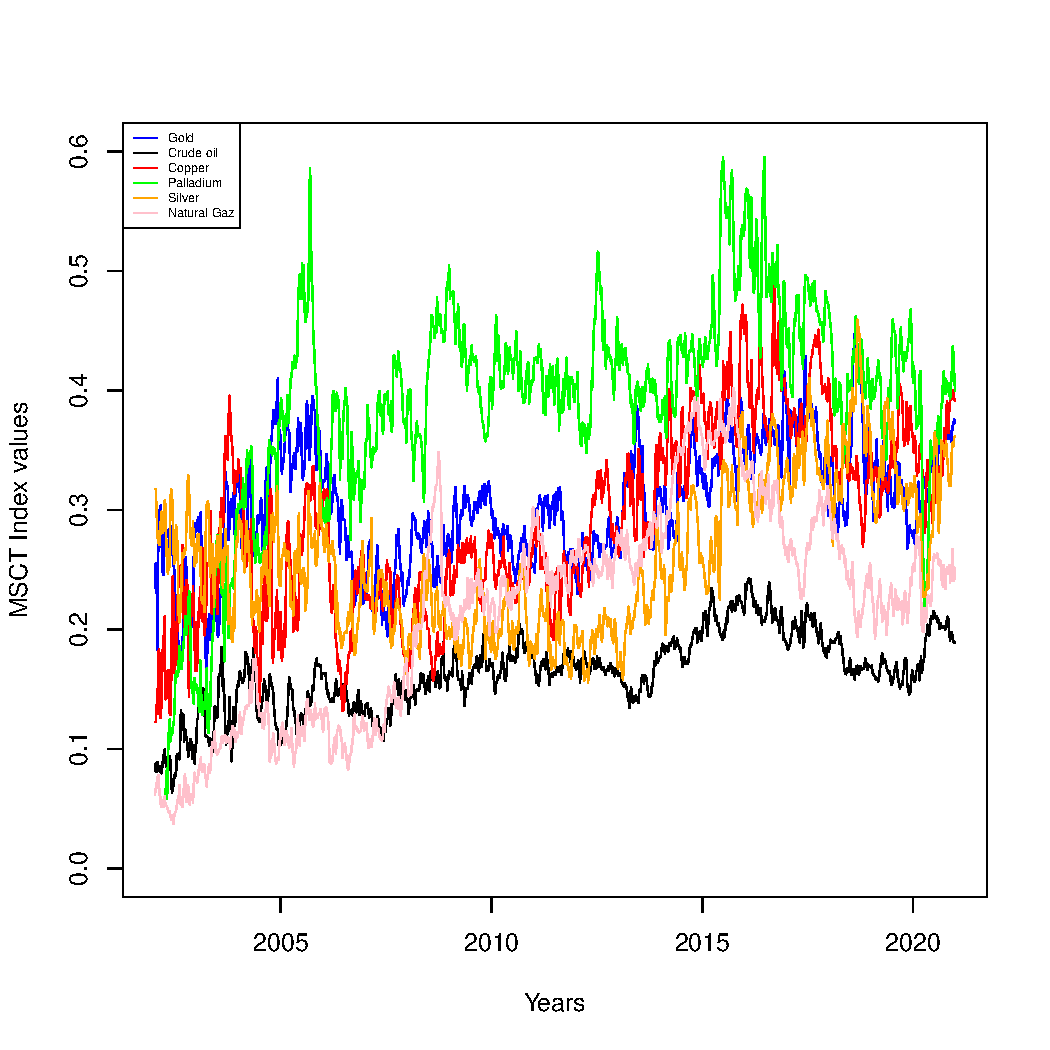
\includegraphics[scale=0.8]{FIG_MSCT}}
		\caption{Time series showing the evolution of the Market Share of Non-Commercials (MSCT) index for all commodities in our sample, 4/2007--12/2020. }
		\label{fig:MSCT}
	\end{figure}


	\begin{figure}[h]
	\centering
		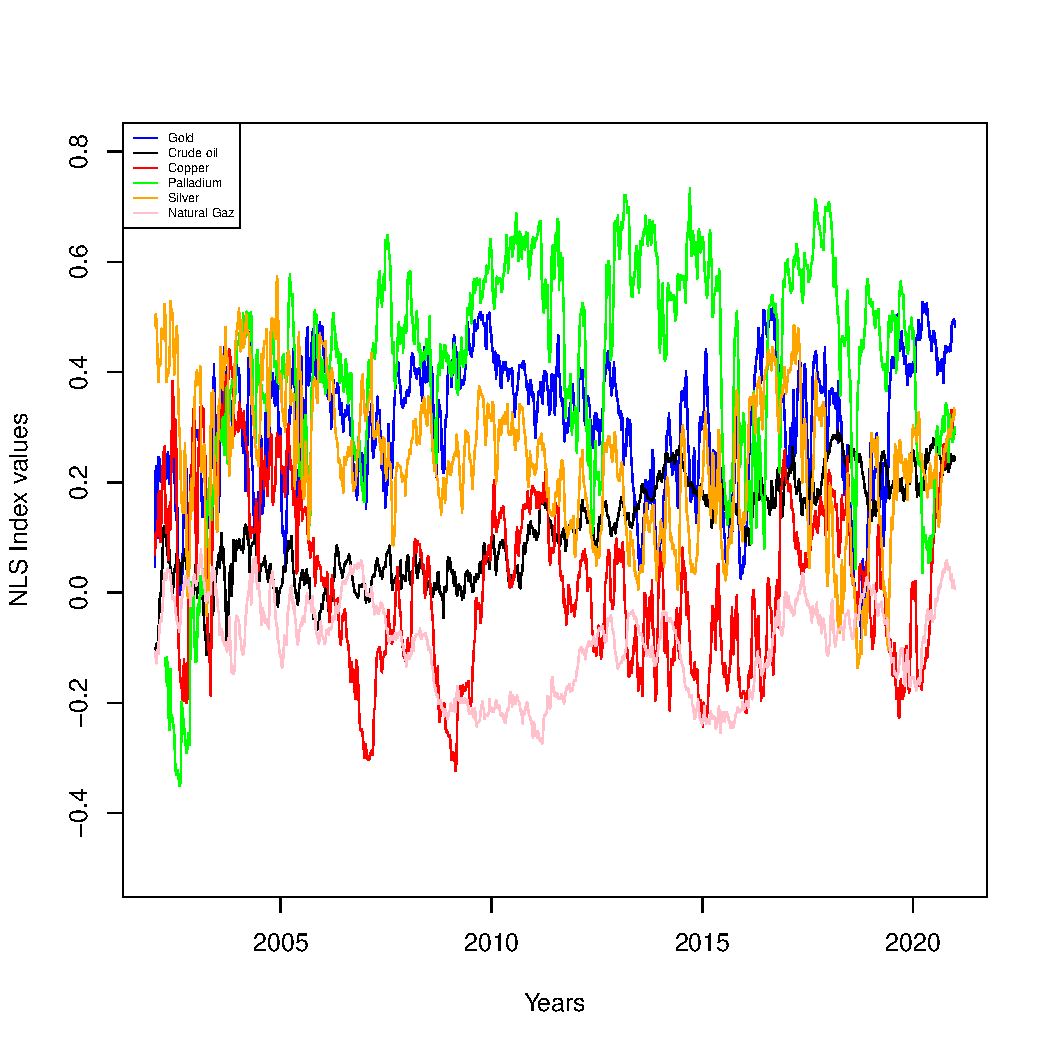
\includegraphics[scale=0.8]{FIG_NLS}}
		\caption{Time series showing the evolution of the Net Long Short (NLS) index for all commodities in our sample, 4/2007--12/2020.}
		\label{fig:NLS}
	\end{figure}

	\begin{figure}[h]
	\centering
		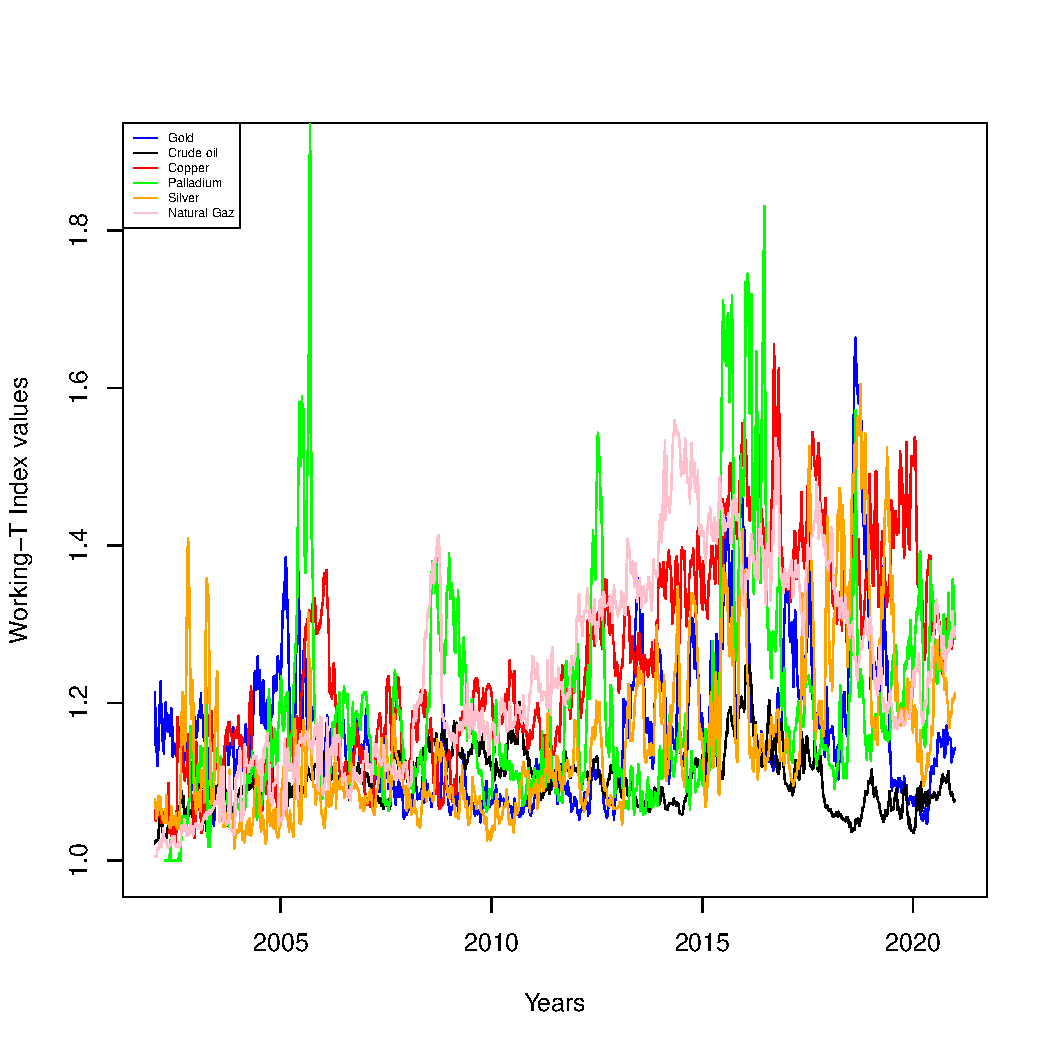
\includegraphics[scale=0.8]{FIG_WT}}
		\caption{Time series showing the evolution of the Working's T index for all commodities in our sample, 4/2007--12/2020.}
		\label{fig:WT}
	\end{figure}
	
\end{document}


